 %% Copyright (C) 2006 Ahmer Ahmedani

\documentclass[MSc,twoside,openright]{Thesis}

\newif\ifdraft
% \drafttrue

%== Preamble ==================================================================

\usepackage[french]{babel}
\usepackage{hhline}
\usepackage[T1]{fontenc}
\usepackage[utf8]{inputenc}
\usepackage{array}
\usepackage{refstyle}
\usepackage{algorithm}
\usepackage{algpseudocode}
\usepackage{placeins}
\usepackage{multirow}
\usepackage{tabularx}
\usepackage{multicol}
\usepackage{xcolor}    % Keyword highlighting in listing
\usepackage{listings}  % Typeset source code listings,
                       % Files in current direcotry
                       % ( listings.cfg listings.sty lstdoc.sty lstlang1.sty
                       % lstlang2.sty lstlang3.sty lstmisc.sty ) are listings
                       % version 1.4, should not be removed, 1.3 version cause
                       % problem in the left line of the frame (standalone use 
                       % of 1.3 will not cause this problem, but in this
                       % project, it does)
\usepackage[bw]{mcode} % mcode listings
\usepackage{x10}			 % x10 listings	
\usepackage{ifthen}    % For conditional commands
\usepackage{ifpdf}     % Provide \ifpdf conditional
\usepackage{xspace}    % Define commands that don't eat spaces
\usepackage{type1cm}
\usepackage{times}     % Use Times *deprecated*
%% listings.sty doesn't seem to pretty print code listings if the
%% `times' packages is not loaded. Why? Who knows. It will do it fine
%% in a simple document, just not in this one.
\usepackage{mathptmx}  % Use Times for roman family and math
% \usepackage{mathpazo}  % Palantino
% \usepackage{chancery}
% \usepackage{bookman}
% \usepackage{newcent}
% \usepackage{charter}
\usepackage[scaled]{helvet}    % Use Helvetica for sans serif family
%\usepackage{avant}     % Use Avant Garde for sans serif family
\usepackage{pifont}    % Symbol and Zapf Dingbats
%% TODO: investigate fourier package (Adobe Utopia fonts)

\usepackage{fancyhdr}  % Fancy page headers
\usepackage{verbatim}  % provide comment environments
\usepackage{fancyvrb}  % improved verbatim and verbatim* environments

%\usepackage{hyperref} % split urls
\usepackage{url}       % For nicely formatted URLs


%% Nicer formatting of figure captions:
\usepackage[format=hang,font={small,sf},labelfont=bf,labelsep=space]{caption}
%\usepackage[tight]{subfigure} % subfigures. replace with subfig?
\usepackage{subfig}
\usepackage{setspace}
\usepackage{longtable} % Make tables span multiple pages
\usepackage{multirow}  % Table cells that span multiple rows
\usepackage{dcolumn}   % Line up decimal sep in tabular columns
% \usepackage{warpcol}   % Alternate to dcolumn
\usepackage{color}     % Allows text and page background colors to be set
\usepackage{colortbl}  % Coloured tables
\usepackage[final]{graphicx}  % Better support for graphics
\usepackage{layout}    % produces a figure that describes the page layout
\usepackage{titlesec}  % to redefine typesetting of \paragraph
\usepackage{rotating}  % for rotated table headings
\usepackage{listings}
\usepackage{stackengine}
% Note: yap does not support rotating, so convert .dvi to .pdf and then
%    preview the .pdf file
% for algorithms
%\usepackage[algo2e, algochapter, ruled, linesnumbered, lined]{algorithm2e}
%% Make sure that the bibliography is listed in the table of contents,
%% but that the table of contents itself is not.
% XXX: doesn't seem to work
%\usepackage[nottoc]{tocbibind} 
\usepackage[none]{tocbibind}
%\usepackage{hyphenat} %enhanced hyphenation, 
%\usepackage[htt]{hyphenat} %htt enables hyphenation of text typeset
% some better colours for hyperref links:
\definecolor{darkgreen}{rgb}{0,0,0}%{0.2,0.5,0.1}
\definecolor{darkblue} {rgb}{0,0,0}%{0.1,0.4,0.5}
\definecolor{maroon}   {rgb}{0,0,0}%{0.45,0.05,0.25}
\definecolor{red}      {rgb}{0,0,0}%{1,0,0}
\ifpdf
  %% TODO: can I use variables here for name, title, etc?
  \usepackage[
    pdftex,
    colorlinks=true,
    linkcolor=maroon,
    citecolor=darkgreen,
    pagecolor=maroon,
    urlcolor=darkblue,
    pdftitle={VeloCty},
    pdfauthor={Sameer Jagdale},
    pdfsubject={The VeloCty compiler},
    pdfkeywords={compiler, C++, static, Velociraptor}
  ]
  {hyperref} % hyper-text links, etc.
\else
  \usepackage[
    dvips,
    breaklinks=true,
    colorlinks=true,
    linkcolor=maroon,
    citecolor=darkgreen,
    pagecolor=maroon,
    urlcolor=darkblue,
  ]
  {hyperref}
\fi


% Use the ams math packages
\usepackage{amssymb,amsmath}

% tell LaTeX where to find find figures
%\ifpdf
%  \DeclareGraphicsExtensions{.pdf,.jpg,.png}
%  \graphicspath{{images/}}
%\else
%  \DeclareGraphicsExtensions{.eps,.ps}
%  \graphicspath{{images/}}
%\fi

\usepackage{bnf}




% -- Customize Layout ---------------------------------------------------------

% custom page headers:

\lhead[]{\fancyplain{}{\nouppercase{\rightmark}}}
\rhead[\fancyplain{}{\nouppercase{\leftmark}}]{}
\addtolength{\headwidth}{10mm} % => extend line out into margin

%\fancyhead[EL]{THESIS DRAFT}
%\fancyhead[OR]{THESIS DRAFT}


\titleformat{\paragraph}[hang]{\normalfont\it}{}{0em}{}

% Make LaTeX relax a little wrt figure placement
\renewcommand{\topfraction}{0.85}
\renewcommand{\textfraction}{0.1}
\renewcommand{\floatpagefraction}{0.75} % Prevent half-empty pages

\newcommand*\justify{%
  \fontdimen2\font=0.4em% interword space
  \fontdimen3\font=0.2em% interword stretch
  \fontdimen4\font=0.1em% interword shrink
  \fontdimen7\font=0.1em% extra space
  \hyphenchar\font=`\-% allowing hyphenation
}
\newcommand{\velocty}{{Velo\textbf{C}ty}\xspace}
\newcolumntype{L}[1]{>{\raggedright\let\newline\\\arraybackslash\hspace{0pt}}m{#1}}
\newcolumntype{C}[1]{>{\centering\let\newline\\\arraybackslash\hspace{0pt}}m{#1}}
\newcolumntype{R}[1]{>{\raggedleft\let\newline\\\arraybackslash\hspace{0pt}}m{#1}}
% Tell LaTeX to not "bottom justify" text. This prevents ugly
% spaces between paragraphs in columns when LaTeX stretches them.
\raggedbottom

% Set the depth for the table of contents to 2 for non-draft output
\ifdraft
\else
\setcounter{tocdepth}{2}
\fi
\lstset{
  basicstyle=\small,
  breaklines=true
  }



\algnewcommand{\Lcomment}[1]{\State \(\triangleright\){\color{gray}{\footnotesize
\textit {#1}}}}
%\ifdraft
%  \pagestyle{myheadings} \markright{Draft \today: Please do not 
%  redistribute.}
%\else
%  \pagestyle{headings}
%\fi

% Set the value of the margin of all algorithms.
% The default value is \leftskip plus \parindent 
%  when the algorithm2e package is loaded. 
%\incmargin{\parindent} %increase one more \parindent to the default 
% Set font of comment in algorithms
\algnewcommand{\algcommentfont}[1]{{\small \texttt{#1}}}
%\SetCommentSty{algcommentfont}

%----------Matlab---------------------
\newcommand{\abc}{\textsl{abc}\xspace}
\newcommand{\amc}{\textsl{amc}\xspace}
\newcommand{\matlab}{{\sc Matlab}\xspace}
\newcommand{\smatlab}{{\sc Matlab}}
\newcommand{\smclab}{\textrm{\textsl{Mc}\textbf{\textsc{Lab}}}}
\newcommand{\mclab}{\smclab\xspace}
\newcommand{\mcirs}{\textrm{\textsl{Mc}\textbf{\textsc{ir}}}}
\newcommand{\smcir}{\mcirs}
\newcommand{\mcir}{\smcir\xspace}
\newcommand{\mcasts}{\textrm{\textsl{Mc}\textbf{\textsc{ast}}}}
\newcommand{\smcast}{\mcasts}
\newcommand{\mcast}{\smcast\xspace}
\newcommand{\smcjit}{\textrm{\textsl{Mc}\textbf{\textsc{jit}}}}
\newcommand{\mcjit}{\smcjit\xspace}
\newcommand{\java}{\textsc{Java}\xspace}
\newcommand{\sjava}{\textsc{Java}}
\newcommand{\fortran}{\textsc{Fortran}\xspace}
\newcommand{\mcbench}{{\sc McBench}\xspace}
\newcommand{\mcfor}{{\sc McFor}\xspace}
\newcommand{\mctwofor}{{\sc Mc2For}\xspace}
\newcommand{\mcsaf}{{\sc McSaf}\xspace}
\newcommand{\kw}[1]{\texttt{#1}}
\newcommand{\xten}{{\sc X10}\xspace}
\newcommand{\mixten}{{\sc MiX10}\xspace}
\newcommand{\parfor}{{\texttt{parfor}}\xspace}
\newcommand{\intok}{{\emph{IntegerOkay}}\xspace}
\newcommand{\rednote}[1]{#1} %{\textcolor{red}{#1}}
\newcommand{\mynote}[1]{} %{\marginpar{\scriptsize{\rednote{#1}}}}
\newcommand{\aspectmatlab}{{\sc AspectMatlab}\xspace}

% MATLAB lang. def. for listings
\lstdefinelanguage{MATLAB}{
    sensitive=true, % Case sensitive identifiers
    morecomment=[l]{\%}, % Line-based comment character
    morestring=[b]', % String character
    morekeywords= {
		function,
		for,
		while,
		if,
		else,
		elseif,
		end,
		aspect,
		patterns,
		actions,
		methods,
		properties,
		class,
		classdef,
		script,
		loops,
		set,
		get,
		call,
		execution,
		mainexecution,
		loop,
		loopbody,
		loophead,
		within,
		before,
		after,
		around
	},
	commentstyle=\color[rgb]{0,0,0}%{.600,.600,.600}, % grey comments
}
% Pseudocode lang. def. for listings
\lstdefinelanguage{pseudo}{
    sensitive=true, % Case sensitive identifiers
    %morecomment=[l]{\#}, % Line-based comment character
    %morestring=[b]', % String character
    morekeywords= {
		function,
		repeat,
		for,
		foreach,
		while,
		if,
		else,
		end,
		equals,
		new,
		add,
		remove,
		return
	},
	commentstyle=\color[rgb]{0,0,0}%{.600,.600,.600}, % grey comments
}

% -- Input local commands and hyphenation rules -------------------------------

% -- Custom Environments ---
\definecolor{darkgrey} {rgb}{0.843,0.843,0.843}
\definecolor{lightgrey} {rgb}{0.979,0.979,0.979}
\lstset{
        language=[AspectJ]Java, %keyword highlighting seems annoying
        morekeywords={declare, parents},
        basicstyle=\ttfamily\footnotesize, % use fixed-width font
        keywordstyle=\bfseries\color[rgb]{.498,.000,.333}, % eclipse color, bold
        %keywordstyle=\bfseries, % bold keywords
        identifierstyle=,       % nothing happens
        %commentstyle=\color[rgb]{.247,.498,.372}, % eclipse color
        commentstyle=\color[rgb]{.753,.753,.753}, % grey comments
        stringstyle=\color[rgb]{.164,.000,1.00},  % eclipse color
        %stringstyle=\ttfamily,  % typewriter type for strings
        showstringspaces=false, % no special string spaces
	    tabsize=2,
        columns=fullflexible,   % Use flexible column format (for comments)
        frame=single, %
        framerule=0.6pt, %
        backgroundcolor=\color{white}, %
        rulecolor=\color{darkgrey}, %
        captionpos=b, %
	    numbers=left, 
	    numberstyle=\scriptsize\color[rgb]{.501,.501,.501},
	    stepnumber=1,
	    breaklines=true,
	    breakatwhitespace=true
}

\newcommand{\code}[1]{{\small \texttt{#1}}}
\newcommand{\codekeyword}[1]{\textbf{\code{#1}}}

% MetaLexer

\newcommand{\mlkw}[1]{\codekeyword{#1}\xspace}
\newcommand{\ml}[1]{\textit{#1}}
\newcommand{\jflexkw}[1]{\codekeyword{#1}\xspace}
\newcommand{\jflex}[1]{\textit{#1}}
%\newcommand{\java}[1]{\textit{#1}}
\newcommand{\weburl}[1]{\textit{#1}}
\newcommand{\file}[1]{\textit{#1}}
\newcommand{\target}[1]{\textit{#1}}
\newcommand{\property}[1]{\textit{#1}}
\newcommand{\cli}[1]{\textit{#1}}
\newcommand{\chapref}[1]{\textit{Chapter \ref{#1}}}
\newcommand{\appendixref}[1]{\textit{Appendix \ref{#1}}}
\newcommand{\sectionref}[1]{\textit{Section \ref{#1}}}
\newcommand{\figref}[1]{\textit{Figure \ref{#1}}}
\newcommand{\tableref}[1]{\textit{Table \ref{#1}}}
\newcommand{\lstref}[1]{\textit{Listing \ref{#1}}}
\newcommand{\lstrefTwo}[2]{\textit{Listings \ref{#1} \& \ref{#2}}}
\newcommand{\lstrefN}[2]{\textit{Listings \ref{#1} - \ref{#2}}}

\newcommand{\secref}[1]{Sec.~\ref{#1}}
\newcommand{\figureref}[1]{Figure~\ref{#1}}
\newcommand{\equationref}[1]{Equation~\ref{#1}}
\newcommand{\eqnref}[1]{(\ref{#1})}
\newcommand{\RC}{reference-counting-based }



\newcommand{\patANY}{\mlkw{<<ANY>>}}
\newcommand{\patEOF}{\mlkw{<<EOF>>}}
\newcommand{\mpatANY}{\mlkw{<ANY>}}
\newcommand{\mpatBOF}{\mlkw{<BOF>}}

\newcommand{\red}[1]{\textcolor{red}{#1}}
\newcommand{\note}[1]{\textcolor{red}{\textbf{#1}}}
\newcommand{\variation}[2]{\textbf{\textcolor{green}{#1} \red{or} \textcolor{blue}{#2}}}

%\newcommand{\mcode}[1]{\lstinline[language=MATLAB]|#1|}
\newcommand{\jcode}[1]{\lstinline[language=Java]|#1|}
\newcommand{\pcode}[1]{\lstinline[language=pseudo]|#1|}


\newcommand{\into}{ 
   \end{minipage}
   \parbox{1cm}{\LARGE\centering $\mathbf{\Rightarrow}$}
   \begin{minipage}{5cm}
 }
\newenvironment{transform}
{
  \begin{center}
    \begin{minipage}{5cm}
}
{
  \end{minipage}
\end{center}
}
\lstnewenvironment{mtrans}
{
\lstset{language=matlab,numbers=none,frame=single}
}
{}

%%% Local Variables:
%%% mode: LaTeX
%%% TeX-master: "thesis"
%%% End: 

% Teach LaTeX how to hyphenate some words

%%% Local Variables:
%%% mode: LaTeX
%%% TeX-master: "thesis"
%%% End: 

\hyphenation{Meta-Lexer}

% -- Andrew's custom header bits -----------------------------------------------------

% Make matlab the default language
\lstset{
  language=MATLAB,
  mathescape=true
}

%== Title Information =========================================================

%--------------------- 70 character title limit -----------------------
\title{VeloCty : an optimizing static compiler for \matlab and Python }

\author{Sameer Jagdale}

\Department{School of Computer Science}
\Institution{McGill University}
\Location{Montr\'eal}

\SubmitDate{}

\CopyrightMessage{Copyright \copyright 2014 Sameer Jagdale}

%== Document ==================================================================

\begin{document}

\pagestyle{empty}

\maketitle
\cleardoublepage

% print a figure describing the current page layout
%\layout

\preface % -- Front Matter ----------------------------------------------------

\begin{Abstract}
abstract
\end{Abstract}

\begin{Resume}
\begin{otherlanguage}{french} 
Les langages scientifiques de haut niveau, tels que MATLAB et Python                                
et sa librairie NumPy, gagnent en popularité auprès des scientifiques                               
et des mathématiciens.  Ces langages offrent des fonctionalités telles                              
que le typage dynamique et des fonctions scientifiques de haut niveau                               
qui permettent un prototypage facile.  Par contre, ces fonctionalités                               
diminue la performance en exécution du code.  

Nous présentons VeloCty,                              
un compilateur statique optimisant pour MATLAB et Python comme                                      
solution au problème d'améliorer la performances des programmes écrits                              
dans ces langages.  Pour la majorité des programmes, une grande                                     
proportion du temps d'exécution est passée à exécuter une petite                                    
section du code.  De plus, ces sections peuvent souvent être compilées                              
avant l'exécution du code et on peut obtenir une amélioration en                                    
performance en optimisant seulement ces sections chaudes.  VeloCty                                  
prend en entrée des fonctions écrites en MATLAB et Python spécifiées                                
par l'utilisateur et génère une version équivalente en C++.  VeloCty                                
génère également le code d'interfaçage pour l'intégration avec MATLAB                               
et Python.  Le code généré peut ainsi être compilé comme une                                        
bibliothèque partagée qui peut être liée avec n'importe quel programme                              
écrit en MATLAB et Python.  Nous implémentons aussi des optimisations                               
pour éliminer les tests de bornes des tableaux, pour réutiliser de la                               
mémoire déjà allouée dans les opérations sur les tableaux, et pour                                  
supporter l'exécution parallèle via OpenMP.                                                         
                                                                                                    
VeloCty utilise le système de compilation Velociraptor.  Nous                                       
implémentons un générateur de code qui transforme la représentation                                 
intermédiaire de Velociraptor, VRIR, en C++ ainsi que des supports                                  
d'exécution spécifiques pour MATLAB et Python.  Nous avons également                                
implémenté un générateur de code MATLAB à VRIR à l'aide de McLab.                                   
                                                                                                    
VeloCty a été évalué avec des programmes de test de performance, 17 écrits en MATLAB et 9 écrits en Python.                              
Les résultats de VeloCty en utilisant toutes nos optimisations sur les                              
tests en MATLAB montrent qu'il est 1.3 à 458 fois plus rapide que                                   
l'interpréteur et le compilateur en-ligne de MATLAB 2014b par                                       
MathWorks.  Pour les tests en Python, VeloCty est 44.11 à 1681 fois                                 
plus rapide que l'interpréteur CPython. 
\end{otherlanguage}


\end{Resume}

\chapter*{Acknowledgements}
I am thankful to my supervisor, Prof. Laurie Hendren, whose help and encouragement has made this thesis possible. It is because of her that I will graduate from the Master's program with a greater understanding  of compilers as well as a greater respect for them . 

I would also like to thank Rahul Garg, who developed the Velociraptor framework on which this research relies heavily upon. Moreover, I would like to thank him for suggesting this line of research and for mentoring me throughout the course of my research. 

Additionally, I would like to thank Vineet Kumar, Ismail Badawi and Xu Li who helped me understand the \mclab framework as well as Erick Lavoie and Vincent Foley-Bourgon who helped me translate the abstract in French. I would also like to thank my other labmates, Sujay Kathrotia, Faiz Khan, Andrew Bodzay and Lei Lopez who made working in the lab fun. 

I would also like to thank my parents, my brother and my all of my friends old and new, who never stopped supporting me and without whom I would not be where I am today.

Finally, I would like to thank the wonderful city of Montreal, whose beauty and people have made my Master's experience magical and memorable. 

This work was supported, in part, by the Natural Sciences and Engineering Research
Council of Canada (NSERC).



\renewcommand{\contentsname}{Table of Contents}%
\addto\captionsenglish{%
  \renewcommand{\contentsname}%
    {Table of Contents}%
}
\addto\captionsenglish{%
  \renewcommand{\lstlistlistingname}%
    {List of Listings}%
}

\tableofcontents
\listoffigures
\listoftables
% Make the 'list of listings' page follow the conventions for the title
\renewcommand{\lstlistlistingname}{List of Listings}
%This line results in a duplicate entry in the .out file
%\renewcommand{\lstlistoflistings}{\begingroup
%  \tocfile{\lstlistlistingname}{lol}
%\endgroup}
\lstlistoflistings 
%\listoflistings
%\listofalgorithmes
\cleardoublepage

\maintext % -- Main Body ------------------------------------------------------

\pagestyle{fancyplain}
%\setcounter{secnumdepth}{3} % Make subsubsections numbered

\chapter{Introduction} \label{chap:Introduction}
With the advent of multicore processors,there has been a renewed interest in the development of performance tools and algorithms targeted for parallel architectures. Many research areas  provide a wide variety of problems which would show improved performance when executed in parallel. One such area is scientific and numerical computing. Scientic algorithms are used by researchers from various fields such as chemistry, biology, geography etc. as well as different sub-fields of computer science like machine learning. In most cases, these algorithms are written in languages  that are collectively known as  array based languages. A few examples of such languages are \matlab\cite{matlab}, Julia\cite{julia} and Python\cite{python} with it's NumPy\cite{numpy} library.\\
Array based languages offer features like, a interpreter style read-eval-print-eval,functions such as eval and feval for dynamic code evaluation,  no types etc. which enable rapid prototyping. However due to the very same features, these languages show poorer performance when compared to statically compiled languages. A common approach for improving the performance is compile whole programs to languages such as {\sc FORTRAN} and C. However, in most cases, the most computationally intensive portion of the program is small, often localised inside a loop body. Hence compiling the entire program is not necessary. In most cases speed up observed through partial compilation of hot code sections is commensurate with that observed by compiling the whole program. This allows the user to continue programming in the language he/she is more comfortable in.\\
This thesis addresses the problem of improving the performance of programs written in array based languages by compiling the hot sections to parallel C++. We support both \matlab\cite{matlab} and Numpy\cite{numpy}. There are two main challenges. First one is supporting the different and often complementary semantics of both languages. The other is supporting the large number of builtins methods that are supported by both languages.
Our solution implement a static C++ backend for velociraptor toolkit and use tools to compile matlab\cite{matlab} and Python\cite{python} programs to the velociraptor intermediate representation. The McLab static pipeline is used for \matlab\cite{matlab} and PyVrir, a Python\cite{python} frontend for Velociraptor is used for Python\cite{python}. 
\section{\velocty compilation pipeline}
The compilation pipeline for \velocty can be seen in \ref{Fig:Overview}. As mentioned earlier, PyVrir is a proof of concept Python\cite{python} frontend that is part of the Velociraptor framework and the \matlab\cite{matlab} frontend is written using the \mclab frontend. In the \mclab pipeline a \matlab\cite{matlab} program is parsed by the \mclab frontend and converted into an AST based representation known as McAST. The McSAF\cite{doherty11} framework then performs various analyses such as kind analyses and function lookup on McAST and then generates another AST based representation called McLAST. The framework also performs a colon2range transformation that was implemented as part of this thesis. Additional details on the colon2range analysis can be found in \chapref{chap:McSAFTranslate}. McLAST is then converted to TameIR\cite{Dubrau:2012} by the Tamer\cite{Dubrau:2012} framework. TameIR\cite{Dubrau:2012} is a three address representation of \matlab\cite{matlab}. Analyses such as value analysis, shape analysis, isComplex analysis and IntegerOk analysis are performed on this IR. These analyses provide information on the type, dimensions and complexity of different variables code which is useful for generating the VRIR and subsequently the C++ code. The IntegerOk analysis identifies variables which can safely be declared as integers in the target language. This analysis is useful since \matlab\cite{matlab} defines all variables as double by default. TameIR\cite{Dubrau:2012} is then given as input to Tamer+, a code aggregation framework, which generates the high-level McLAST representation from it. Code generated from McLAST is devoid of temporary variables and hence has better readability.The VRIR code generator takes McLAST as input and generates VRIR in the s-expression format. It also generates, glue code using the \matlab\cite{matlab} Mex\cite{mex} API which is required for interfacing with \matlab\cite{matlab}.\\ 
The VRIR is then parsed by the Velociraptor frontend and converted into an AST representation. Various passes such as the simplification pass, loop info collector and the index info collector pass are performed over the AST and is then passed to the static code generator. Finally, the code generator outputs C++ code which can then be compiled to a shared library along with the language specific run time library containing helper functions and the glue code. 
\begin{figure}[htbp]
\begin{center}
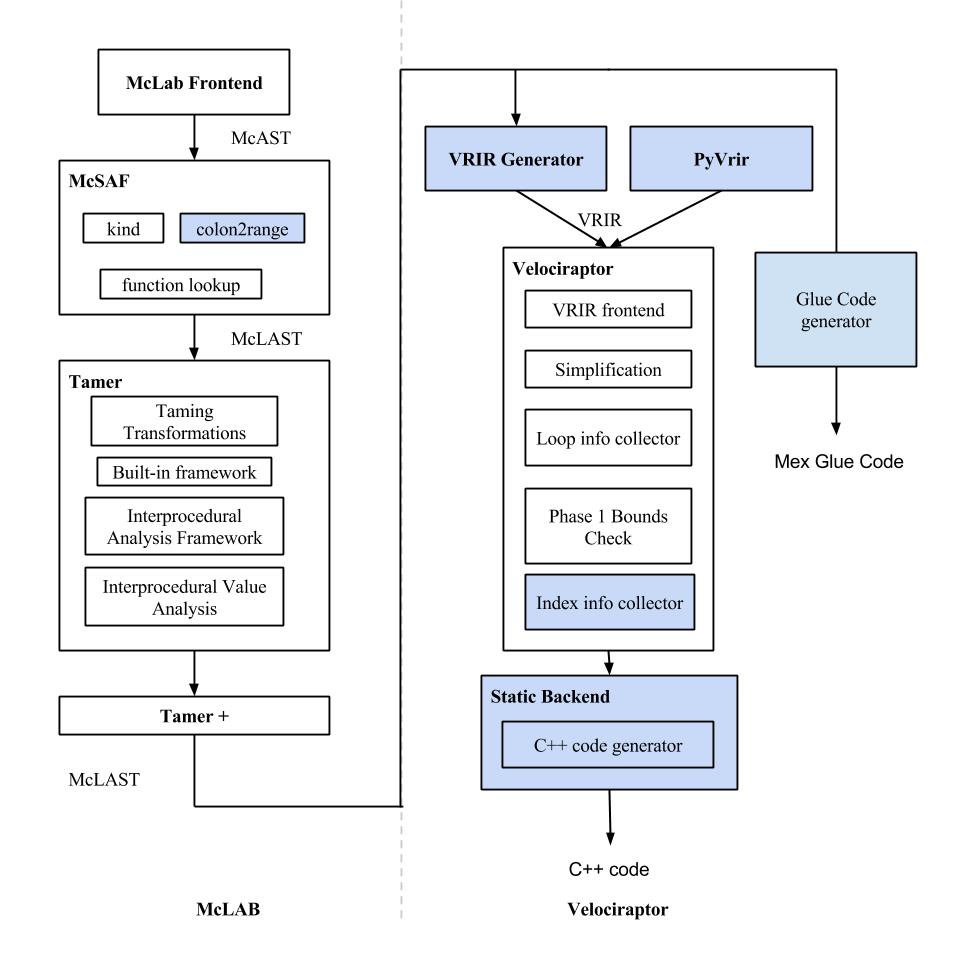
\includegraphics[scale=0.5]{Figures/Overview_thesis.png}
\caption[Overview of the VeloCty]{Overview
of VeloCty. The shaded boxes indicate the components
presented in this thesis. The other solid boxes correspond to
existing \mclab and Velociraptor tools we use}\label{Fig:Overview}
\end{center}
\end{figure}
\section{The Execution Model} 

\begin{figure}[htbp]
\begin{center}
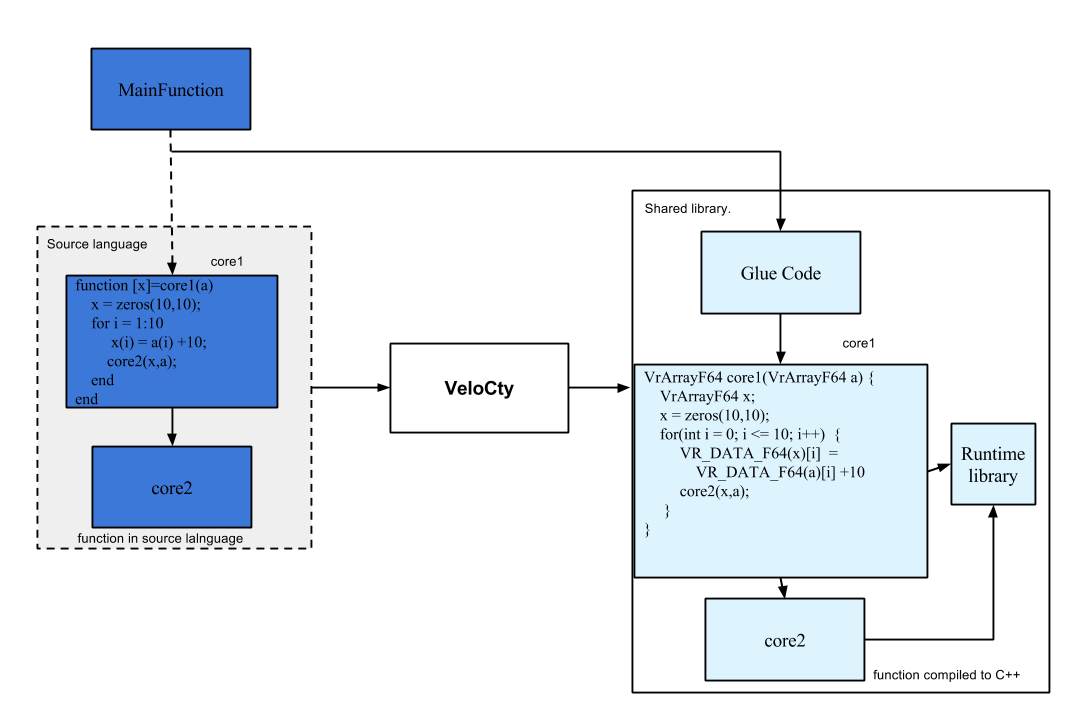
\includegraphics[scale=0.4]{Figures/WorkingDetails.png}
\caption[Execution Model]{Execution model of VeloCty.}\label{Fig:working}
\end{center}
\end{figure}
\section{Contributions}
The main contributions of this thesis are as follows.
\begin{itemize}
\item Generating the velociraptor intermediate representation from the McSAF\cite{doherty11} intermediate representation. 
\item Implementation of a transformation from  Colon expressions to Range expressions
\item Generating glue code necessary for invoking C++ functions from \matlab\cite{matlab}.
\item Generating C++ code from the Velociraptor IR.
\item Optimizing generated code by elminating bounds checks unncessary memory allocations. 
\end{itemize}
\section{Thesis Outline}
This thesis is divided into \ref{chap:Conclusions} chapters, including this one, which are structured as follows.
\chapref{chap:Background} gives a brief overview of the tools
used by VeloCty.
\chapref{chap:McSAFTranslate} describes the translation from the McSAF\cite{doherty11}.
intermediate representation to the Velociraptor intermediate representation(VRIR).
\chapref{chap:glueCode} describes the various aspects of generating glue code for \matlab\cite{matlab}'s Mex API including how input data is converted from Mex data structures to VeloCty data structures. 
\chapref{chap:vrirBackend} talks about the generation of C++ code from VRIR.
\chapref{chap:codeOptimise} explains the code optimisations implemented to improve the performance. 
\chapref{chap:Related} provides an overview of related work and
\chapref{chap:Conclusions} concludes.

\chapter{Background} \label{chap:Background}
\velocty can compile functions written in \matlab and NumPy to C++. The compilation process uses different toolkits such as Velociraptor, \mclab etc. Moreover, it was also necessary for us to understand the semantics of \matlab and NumPy to ensure that the generated C++ code semantically matches the code written in the source language. Additionally, we used C API provided by \matlab and Python to interface the generated code with the source language. This chapter discusses the different toolkits and APIs that were used to develop \velocty. We also compare the semantics of \matlab and NumPy which were important for the implementation of the compiler. 
\section{Comparison of Matlab and NumPy semantics}
Our compiler supports two languages, namely \matlab and NumPy. In order to ensure that the code generated matches the semantics of the language from which it was generated, we studied the semantics of both languages. This section discusses the similarities and differences of both languages. 
\subsection{Array Indexing}
\matlab supports 1-indexing, that is the array index starts from 1. 
The array layout is always column major. The upper bound of the index value depends on the number of indices provided. If the number of indices are greater than or equal to the number of dimensions of the array, the maximum value of an index is the size of the dimension. The number of indices can execeed the number of dimensions of the array as long as all the indices greater than the number of dimensions are one. If the number of dimensions of 
\subsection{Bounds checks}
\subsection{Builtins functions}
\section{C APIs}
We used the C APIs provided by \matlab and Python to interface the generated code with the source language. To interface with \matlab, we use the MEX\cite{mex} API and the Python C API is used for Python. 
\subsection{MEX}
The Mathworks' MEX provides functions and data structures to allow interfacing code in \matlab with code in C/C++. In order to use these functions, the \textsf{mex.h} header file is required to be included. A compiler to  compile the C/C++ code is also provided. Data between the \matlab code and the C++ code is passed as pointers to MxArrays. The raw array data and meta data can be accessed through different MEX functions. MEX also provides functions to create and destroy MxArrays as well as other basic memory management functions. Table \ref{tab:mexFunc} gives a list of MEX functions that are used for interfacing with the source langauge. 
\begin{table}[h]
\centering
\begin{tabular}{|c|c|}
\hline
MEX Functions           & Description                                                                                                                                                   \\ \hline
mxCreateNumericArray    & \begin{tabular}[c]{@{}c@{}}Creates an MxArray given dimensions, \\ number of dimensions, element type\\ and whether the array is real or complex\end{tabular} \\ \hline
mxCreateDoubleScalar    & \begin{tabular}[c]{@{}c@{}}Creates an MxArray with a single \\ element of type double.\end{tabular}                                                           \\ \hline
mxDestroyArray          & Frees memory allocated to the MxArray                                                                                                                         \\ \hline
mxMalloc                & Allocates memory of specified size in bytes                                                                                                                   \\ \hline
mxFree                  & Frees memory allocated by                                                                                                                                     \\ \hline
mxGetData               & \begin{tabular}[c]{@{}c@{}}Returns a void pointer to the raw array data\\ of a MxArray\end{tabular}                                                           \\ \hline
mxSetData               & \begin{tabular}[c]{@{}c@{}}Sets the mxArray's data pointer to given \\ memory.\end{tabular}                                                                   \\ \hline
mxSetDimensions         & \begin{tabular}[c]{@{}c@{}}Sets the dimensions and number of \\ dimensions of a mxArray\end{tabular}                                                          \\ \hline
mxGetDimensions         & Returns the dimensions of a mxArray                                                                                                                           \\ \hline
mxGetNumberOfDimensions & Returns the number of dimensions of a mxArray                                                                                                                 \\ \hline
\end{tabular}
\caption[List of MEX functions]{The table lists the MEX functions that were used by \velocty.}
\label{tab:mexFunc}
\end{table}

The entry point function for MEX is known as mexFunction. Every C/C++ program that is to be interfaced with \matlab is required to have an implementation of the  mexFunction. Listing \ref{lst:mexFunction} gives  the function signature of the mexFunction. The mexFunction takes four input parameters. The first parameter, \textsf{nlhs} defines the number of output parameters. The second paramater \textsf{plhs} is an array of mxArray pointers. \textsf{plhs} holds the output parameters of the function. The third and fourth parameters, \textsf{nrhs} and \textsf{prhs}, define the number of input parameters and the input parameters of the function. All elements of the plhs array are set to NULL and hence mxArrays need to created in the C/C++ code before the function returns. On the other hand, prhs contains the input mxArrays that have been created by the calling function. 
\begin{lstlisting}[float,language=lisp, label={lst:mexFunction}, caption={Function signature of mexFunction}]
void mexFunction(int nlhs, mxArray *plhs[], int nrhs, 
  const mxArray *prhs[])
\end{lstlisting}

The C/C++ program can then be compiled using the MEX compiler. The compiler generates a dynamically linked library having the same name as the C/C++ source file. The MEX C/C++ function can then be called from a \matlab program as a regular \matlab function. 

\subsection{C APIs for Python}
Programs written in C/C++ can be interfaced with Python using the Python/C API. We also use the NumPy/C API passing and returning arrays. The data structures and functions provided to interface with Python can be used by including the header file \textsf{Python.h}.In order to interface with Python code, the C/C++ has to be structured as a Python module. 
A Python program passes data to the C/C++ program as a single parameter, which is a pointer to a PyObject. If multiple paramaters are to be passed into the function, the PyObject may represent an array of other PyObjects. Unlike MEX, there is no restriction on the name of the entry point function. Listing \ref{lst:pyFunc} gives an example of a C function which serves as an entry point function. The static function, arc\_distance, returns a pointer to a PyObject and take two input parameters, both PyObject pointers. The first input parameter, \textsf{self} is a pointer to the module object. The second parameter, \textsf{args} contains the input arguments of the function. 
\begin{lstlisting}[float,language=C, label={lst:pyFunc}, caption={Signature of a function that can be called from Python}]
  static PyObject* arc_distance(PyObject* self, PyObject *args); 
\end{lstlisting}

The methods that can be accessed from Python in the given module have to listed in an array of structs of the type PyMethodDef. PyMethodDef has four fields: method name as a string, pointer to the method implementation, METH\_VARGS which tells Python how to access the method and finally the documentation for the method. The last entry into the array should have all NULL values to indicate the end of the array. Listing \ref{lst:pyMethod} gives an example of the PyMethodDef array for the function arc\_distance. 
\begin{lstlisting}[language=C, label={lst:pyMethod}, caption={An Example of the PyMethodDef struct }]
static PyMethodDef arc_distance_kernelMethods[] =
   {
       {"arc_distance",arc_distance,METH_VARARGS,"arc_distance of a circle. "},
       {NULL,NULL,0,NULL}
   };
\end{lstlisting}

Additionally, a struct of type PyModuleDef also needs to be initialised. PyModuleDef describes the module. Listing \ref{lst:pyModule} gives an example of the PyModuleStruct for the module arc\_distance. The struct holds module information such as the name of the module, documentationand the PyMethodDef array among others.
\begin{lstlisting}[language=C, label={lst:pyModule}, caption={Example of the PyModuleDef struct}]
 static struct PyModuleDef arc_distance_kernelModule = {
       PyModuleDef_HEAD_INIT,
       "arc_distance_kernelModule",
       NULL,
       -1,
      arc_distance_kernelMethods,
  };
\end{lstlisting}

 Finally, the C/C++ program is required to implement the module initialisation function. Listing \ref{lst:pyInit} gives an example of the initialisation function. The name of the function is PyInit\_<module name>, that is \textsf{PyInit\_} followed by the name of the module. In this case the name of the module is arc\_distance. A module object is initialised using the method PyModule\_Create which takes the PyModuleDef struct as input. The function import\_array, is used to initialise NumPy specific constructs. 
\begin{lstlisting}[language=lisp, label={lst:pyInit}, caption={Example of the module initialisation function for the module arc\_distance}]
 PyMODINIT_FUNC
   PyInit_arc_distance_kernel(void){
        PyObject* m = PyModule_Create(&arc_distance_kernelModule);
       import_array();
       return m;
   }

\end{lstlisting}
\section{\mclab}
\mclab is an extensible compiler toolkit for \matlab. \mclab provides compilation, analysis and execution tools to optimise \matlab. \mclab provides frameworks to aid static compilation of \matlab programs to other languages such as Fortran and X10. These tools provide analyses which aid easy compilation of \matlab programs to different targets. McSAF, Tamer and Tamer+ are the three frameworks that are used for implementing static compilers for \matlab. 
\subsection{McSAF}
McSAF is a static analysis framework for implementing static analyses for the \matlab language. McSAF provides APIs and the core functionality to impelent static analyses with ease. It also provides an intermediate representation known as McLAST on which the analyses and transformations can be performed. McLAST is a high-level AST\footnote{Abstract Syntax Tree} based representation with a structure close to the \matlab program from which it was generated. McSAF can be used for various purposes such as static compilation to static and dynamic languages, code refactoring etc. 

The kind analysis\cite{Doherty:2011:KAM:2076021.2048077}, implemented using McSAF, separates array index operations from function calls. This analysis is crucial because both array index operations and function calls are syntactically similarly and hence can not be differentiated statically based on syntax alone. 

The colon expression to range expression transformation was also performed using the McSAF framework. This transformation was a contribution on this thesis and is explained in Section \ref{sec:colonExpr}. 

Table \ref{tab:mcsaf} gives an example of a \matlab function babai, and the equivalent McSAF code that was generated. As we can observe, the generated McSAF code is very close to the original \matlab function. 
\begin{table}[htbp]
\centering
\begin{tabular}{|l|l|}
\hline

\matlab & McSAF \\
\hline
{
\begin{lstlisting}[language=matlab,frame=none, numbers=none]
function z_hat = babai(R,y)
n=length(y);
z_hat=zeros(n,1);
z_hat(n)=round(y(n)./R(n,n));

for k=n-1:-1:1
    par=R(k,k+1:n)*z_hat(k+1:n);
    ck=(y(k)-par)./R(k,k);
    z_hat(k)=round(ck);
end

end

\end{lstlisting}
}
&
{
\begin{lstlisting}[language=matlab,frame=none, numbers=none]
function [z_hat] = babai(R, y)
  n = length(y);
  z_hat = zeros(n, 1);
  z_hat(n) = round((y(n) ./ R(n, n)));
  for k = ((n - 1) : (-1) : 1)
    par = (R(k, ((k + 1) : n)) * 
			z_hat(((k + 1) : n)));
    ck = ((y(k) - par) ./ R(k, k));
    z_hat(k) = round(ck);
  end
end
\end{lstlisting}

}
 \\
\hline
\end{tabular}
\caption[Example of a \matlab function and the equivalent McSAF code. ]{The Table gives an example of a \matlab function babai and the generated McSAF code. }
\label{tab:mcsaf}
\end{table}
\subsection{Tamer}
Similar to McSAF, Tamer is an object oriented toolkit to implement analyses and transformations on \matlab. Tamer facilitates the static compilation of \matlab programs to different static languages. 

Given an entry point function, Tamer generates a complete callgraph. It also handles the large number of \matlab builtins through the Builtin framework.For every function in the callgraph, Tamer converts the function's McSAF intermediate representation, McLAST and genenerates Tame IR, as three address code\footnote{In a three address code based IR, each statement as at most three operands} based intermediate representation with specialised AST nodes. 

Tamer implements analyses on Tame IR which aids static compilation. These include the value analysis which estimates \matlab types, the shape analysis\cite{Li:2014} which infers the dimensions of the variables and the IntegerOkay\cite{vkumar14} which identifies the variables having integer types. 

Table \ref{tab:tamer} gives an example of a \matlab function and the equivalent Tamer code. As we can see, since every statement is broken down into three address code, the length of the generated Tame IR code is quite large.Moreover, we can also observe that operators like \textsf{+}, \textsf{-} have been replaced by function calls. This is because in \matlab, operators are syntactic sugar and are replaced by function calls during execution. 

\begin{table}[htbp]
\centering
\begin{tabular}{|l|l|}
\hline

\matlab & McSAF \\
\hline
{
\begin{lstlisting}[language=matlab,frame=none, numbers=none]
function z_hat = babai(R,y)
n=length(y);
z_hat=zeros(n,1);
z_hat(n)=round(y(n)./R(n,n));

for k=n-1:-1:1
    par=R(k,k+1:n)*z_hat(k+1:n);
    ck=(y(k)-par)./R(k,k);
    z_hat(k)=round(ck);
end

end

\end{lstlisting}
}
&
{
\begin{lstlisting}[language=matlab,frame=none, numbers=none]
function  [z_hat] = babai(R, y)
  [n] = length(y);                    
  mc_t20 = 1;                        
  [z_hat] = zeros(n, mc_t20);        
  [mc_t3] = y(n);                    
  [mc_t4] = R(n, n);                 
  [mc_t2] = rdivide(mc_t3, mc_t4);   
  [mc_t0] = round(mc_t2);            
  z_hat(n) = mc_t0;                  
  mc_t21 = 1;                        
  [mc_t18] = minus(n, mc_t21);       
  mc_t22 = 1;                        
  [mc_t19] = uminus(mc_t22);         
  mc_t25 = 1;                        
  for k = (mc_t18 : mc_t19 : mc_t25);
    mc_t10 = k;                       
    mc_t23 = 1;                       
    [mc_t12] = plus(k, mc_t23);       
    mc_t13 = n;                       
    [mc_t11] = colon(mc_t12, mc_t13); 
    [mc_t5] = R(mc_t10, mc_t11);      
    mc_t24 = 1;                       
    [mc_t8] = plus(k, mc_t24);        
    mc_t9 = n;                        
    [mc_t7] = colon(mc_t8, mc_t9);    
    [mc_t6] = z_hat(mc_t7);           
    [par] = mtimes(mc_t5, mc_t6);     
    [mc_t16] = y(k);                  
    mc_t17 = par;                     
    [mc_t14] = minus(mc_t16, mc_t17); 
    [mc_t15] = R(k, k);               
    [ck] = rdivide(mc_t14, mc_t15);    
    [mc_t1] = round(ck);    
    z_hat(k) = mc_t1;        
  end
end
\end{lstlisting}

}
 \\
\hline
\end{tabular}
\caption[Example of a \matlab function and the equivalent Tame IR code. ]{The Table gives an example of a \matlab function babai and the generated Tame IR code. }
\label{tab:tamer}
\end{table}
\section{Tamer+}
Tamer+ is a code aggregation framework. Since Tame IR is a three address code based IR, the code generated from Tame IR is long  and not human readable, due to the use of temporary variables. Hence, in order to improve code readability, Tamer+ aggregates multiple statements together and reduces the number of statements. Tamer+ takes as input Tame IR and outputs McSAF IR (McLAST). The generated code has fewer statements and is hence more readable.

Table \ref{tab:tamer+} gives an example of a \matlab function and the equivalent McSAF code generated from Tame IR by Tamer+. The code length is almost the same as the original \matlab function. 
\begin{table}[htbp]
\centering
\begin{tabular}{|l|l|}
\hline

\matlab & McSAF(Generated by Tamer+) \\
\hline
{
\begin{lstlisting}[language=matlab,frame=none, numbers=none]
function z_hat = babai(R,y)
n=length(y);
z_hat=zeros(n,1);
z_hat(n)=round(y(n)./R(n,n));

for k=n-1:-1:1
    par=R(k,k+1:n)*z_hat(k+1:n);
    ck=(y(k)-par)./R(k,k);
    z_hat(k)=round(ck);
end

end

\end{lstlisting}
}
&
{
\begin{lstlisting}[language=matlab,frame=none, numbers=none]
function [z_hat] = babai(R, y)
  [n] = length(y);
  [z_hat] = zeros(n, 1);
  z_hat(n) = round(rdivide(y(n), R(n, n)));
  for k = (minus(n, 1) : uminus(1) : 1);
    [par] = mtimes(R(k, colon(plus(k, 1), n)), z_hat(colon(plus(k, 1), n)));
    [ck] = rdivide(minus(y(k), par), R(k, k));
    z_hat(k) = round(ck);
  end
end
\end{lstlisting}

}
 \\
\hline
\end{tabular}
\caption[Example of a \matlab function and the equivalent McSAF code generated by Tamer+ . ]{The Table gives an example of a \matlab function babai and the generated McSAF code generated from Tame IR by Tamer+. }
\label{tab:tamer+}
\end{table}
\section{Velociraptor}
Velociraptor is a compiler toolkit aimed at improving performance of array-based languages such as \matlab and NumPy. The toolkit consists of an intermediate representation known as VRIR. The toolkit also provides various analysis on transformation on the IR. A compiler known as PyVrir, for Python to VRIR is also provided. 
\subsection{VRIR}
VRIR is high-level strongly typed AST based intermediate representation. VRIR is designed to be flexible to accomodate semantics of different scientific languages such as \matlab and Python's NumPy library. VRIR supports various array indexing schemes such as 0-indexing, 1-indexing and negative indexing and multiple array layouts such as row major, column major and stride major. VRIR also supports parallelism through constructs such as parallel for loop, map and reduce etc. VRIR can be generated as a string in the s-expression format which will then be converted to a C++ based AST. Alternatively, the C++ AST can directly be generated.


\subsection{Parser}
If a language frontend compiling to VRIR, generates VRIR in the s-expression format and dumps it in a file, this file can be given to a parser implemented using Antlr\footnote{Information about Antlr can be found here \url{http://www.antlr3.org/}}. The parser generates an Antlr AST which is then converted into a C++ VRIR AST. This AST is then used for optimisations and code generation.  
\subsection{Analyses}
The Velociraptor toolkit also performs analyses and optimisations on VRIR which  can be resusable across compiler backends. The simplification pass simplifies expressions containing array operations into a three address code format. This simplification was useful to us while implementing the memory optimisation described in Section \ref{sec:memoptimise}. The preliminary bounds check eliminations analysis, identifies and eliminates redundant bounds checks.


\chapter{Generating VRIR from the  McSAF Intermediate Representation} \label{chap:McSAFTranslate}
As mentioned in the earlier chapters, \velocty supports \matlab and Python's NumPy library. The \velocty backend takes VRIR as input and generates C++ code. We use PyVrir that is part of the Velociraptor toolkit generate VRIR from Python. However, no such tool exists to generate VRIR from \matlab to VRIR. The \mclab toolkit is a framework to aid static compilation of \matlab to different languages. In order to support the compilation of \matlab programs to C++ through \velocty, we implemented a VRIR generator using the \mclab toolkit. Section \ref{sec:comppipe} provided an overview of the compilation pipeline from \matlab to VRIR and then to C++. As mentioned in the section, the VRIR generator takes an input McSAF IR and generates the S-expression version of VRIR.

VRIR generation had challenges. The McSAF IR is a \matlab-specific IR whereas VRIR is designed to handle semantics of different languages and thus contains flags to specify semantic information such as array layout, indexing scheme etc. We had to ensure the appropriate flags were set to correctly represent the semantics of \matlab. Moreover, VRIR is a strongly typed AST representation. Every expression node in VRIR has a type and shape information associated with it. McSAF does not explicitly hold this information and hence had to be determined during the compilation process. Additionally, \matlab functions do not need an explicit return statement for the output. When a return statement is explicitly provided, the parameters that need to be returned are not specified. This is because the output parameters are specified in the function signature. On the other hand, VRIR does not support output parameters and only supports output types. This difference in IR structure also had to be handled.

This chapter discusses the compilation of various nodes of the McSAF IR to VRIR, generation of the symbol table and how the types and shapes of expressions are determined.
\section{Mapping types}
In order to generate VRIR types, we require type and shape information as well as whether the symbol is real or complex. This information is obtained through the type analysis , the shape analysis and the isComplex analysis that were performed on Tamer. All variables and expressions are mapped to one of 5 VRIR types which are collectively known as VTypes.


\subsection{Scalar Type}
Scalar types are used for scalar symbols. In this case the shape of the symbol will have two dimensions each of size one. The scalar type also as a \textsf{ctype} flag which determines whether the symbol is real or complex. The symbol is considered to be real if the flag is set to zero and complex if it is set to one. The type of the data also needs to be specified in the generated VRIR. Types in \matlab are known as MClasses. Table \ref{tab:mclassList} gives a list of MClasses that are supported by the VRIR generator. Note that the VRIR generator does not support other MClasses such as \textsf{char}, unsigned integers and 16 and 8 bit integers. 
\begin{table}[htbp]
\centering
\begin{tabular}{|c|c|c|}
\hline
MClass  & VRIR Scalar Type & Description           \\ \hhline{|=|=|=|}
Logical & bool &Boolean type          \\ \hline
Int32   & int32 &32 bit Integer        \\ \hline
Int64   & int64 &64 bit Integer        \\ \hline
Float32 & float32 & 32 bit Floating point \\ \hline
Float64 & float64 & 64 bit Floating point \\ \hline
\end{tabular}
\caption[List of \matlab types]{The table lists the different \matlab types known as MClasses  that are supported by the VRIR generator and the Scalar types generated in VRIR.}
\label{tab:mclassList}
\end{table} 

Table \ref{tab:scalTypeMat} gives an example of VRIR for the scalar type from a \matlab variable \texttt{x}.  The example describes a scalar symbol that is of type \textsf{float64} and is \textsf{real}. 
\begin{table}[htbp]
\centering
\begin{tabular}{|l|l|}
\hline

\matlab &  Generated VRIR \\
\hline
{
\begin{lstlisting}[language=matlab,frame=none, numbers=none]
x = 0;
\end{lstlisting}
}
&
{
\begin{lstlisting}[language=lisp,frame=none, numbers=none]
(float64 :ctype 0)
\end{lstlisting}
} \\
\hline
\end{tabular}
\caption[Scalar Type example for \matlab]{The table shows an example of the generated scalar type for a scalar variable x in \matlab. }
\label{tab:scalTypeMat}
\end{table}
\subsection{Array Type}
The array type is used to represent types for \matlab arrays. Arrays can have two or more dimensions and at least one of the dimension sizes have to be greater than one. Note that although \matlab considers scalars to be 1x1 matrices, we make the distinction between scalars and arrays. Shape information is used to determine whether the symbol is an array or a scalar. Array types of VRIR contain information about the number of dimensions of the array and the array layout. The array layout can be \textsf{rowmajor}, \textsf{colmajor} and \textsf{strided}. However, in case of \matlab the layout is always \textsf{colmajor}. Array Types also contain a child node of scalar type. The scalar type holds information about the type of the array elements as well as whether they are \textsf{real} or \textsf{complex}. Table \ref{tab:arrTypeMat} gives an example of the generated array type. The example shows a variable that is assigned to a 3x3 matrix of using the zeros builtin function. The generated VRIR array type contains a ndims attribute which is set to 2 since there are two dimensions, and the array layout attribute is set to colmajor since all arrays in \matlab are column major. Using the child scalar type node of the array type, we can determine that each element of the array is of type \textsf{float64} and that each element is \textsf{real}. 

\begin{table}[htbp]
\centering
\begin{tabular}{|l|l|}
\hline

\matlab &  Generated VRIR \\
\hline
{
\begin{lstlisting}[language=matlab,frame=none, numbers=none]
x = zeros(3,3);
\end{lstlisting}
}
&
{
\begin{lstlisting}[language=lisp,frame=none, numbers=none]
(arraytype :layout colmajor :ndims 2
		(float64 :ctype 0)
)
\end{lstlisting}
} \\
\hline
\end{tabular}
\caption[Array Type example for \matlab]{The table shows an example of the generated array type for an array variable x in \matlab. }
\label{tab:arrTypeMat}
\end{table}
\subsection{Void Type}
The void type is generally used as part of the Function type to convey the absence of the input or output parameters.
\subsection{Function Type}
\label{subsec:functypeMat}
Function types are associated with function definitions and function handles. They contain information about the types of the input and output parameters of the function. The \textsf{functype} node contains two child nodes, \textsf{intypes} and \textsf{outtypes}. Both nodes will have children that can be other VTypes such as scalar types, array types etc. The function types are part of the function node of VRIR. Table \ref{tab:funcTypeMat} gives an example of the Function type generated for the function babai. The function accepts two input parameters both of which are arrays and returns another array. The types of the input arguments are listed inside the intypes child whereas the output parameters are listed inside outtypes. Note that the body of the function is replaced by a statement inside chevrons which acts as a place holder. 
\begin{table}[htbp]
\centering
\begin{tabular}{|l|l|}
\hline

\matlab &  Generated VRIR \\
\hline
{
\begin{lstlisting}[language=matlab,frame=none, numbers=none]
function [z_hat] = babai(R,y) 
<Function Body> 
end;
\end{lstlisting}
}
&
{
\begin{lstlisting}[language=lisp,frame=none, numbers=none]
(functype
	(intypes
		( arraytype :layout colmajor :ndims 2
			(float64 :ctype 0)
		)
		( arraytype :layout colmajor :ndims 2
			(float64 :ctype 0)
		)
	)
	(outtypes
		( arraytype :layout colmajor :ndims 2
			(float64 :ctype 0)
		)
	)
)
\end{lstlisting}
} \\
\hline
\end{tabular}
\caption[Func Type example for \matlab]{The table shows an example of the generated func type for the function babai in \matlab. }
\label{tab:funcTypeMat}
\end{table}
\subsection{Tuple Type}
Tuple types are used to define data structures which can have data of different types. Table \ref{tab:tupletype} gives an example of the tuple type. The table shows a function call to \textsf{spqr} which has multiple returns. The function call expression as well as the expression on the LHS will both have tuple types. In this case the tuple type specifies that the two variables being returned have VTypes, scalar type and array type respectively. 
\begin{table}[htbp]
\centering
\begin{tabular}{|l|l|}
\hline
\matlab &  generated VRIR\\
\hline
{
\begin{lstlisting}[language=matlab,frame=none, numbers=none]
[nc, r]  = spqr(a,tol,maxrc)
\end{lstlisting}
}
&
{
\begin{lstlisting}[language=lisp,frame=none, numbers=none]
(tupletype
	(float64 :ctype 0)
	(arraytype :layout colmajor :ndims 2
		(float64 :ctype 0)
	)
)
\end{lstlisting}
} \\
\hline
\end{tabular}
\caption[Example of the Tuple Type]{The table gives an example of a call to a function with multiple returns in \matlab and the equivalent VRIR tuple type that is generated.}
\label{tab:tupletype}
\end{table}

\subsection{Domain Type}
The domain type is associated with the domain expression explained in Subsection \ref{subsec:domainExprfront}. Domain expressions themselves are only associated with For or parallel For loop statements. Domain types specify the types of all the iterator variables of the loop statements. The domain type has an attribute ndims which specifies the number of iteration variables of the loop. In case of \matlab, there can only be one iteration variable per loop. Listing \ref{lst:domaintype} gives an example of a domain type for a single iteration variable that is of type \textsf{float64}. 
\begin{lstlisting}[language=lisp, label={lst:domaintype}, caption={An example of the domain type in VRIR. }]
(domaintype :ndims 1 (float64 :ctype 0))
\end{lstlisting}

\section{Symbol Table}
The symbol table contains a list of symbols that are defined inside a function in VRIR. The table contains the name and the type of each symbol. Moreover, there is a unique id associated with every symbol using which it is referenced in the function. There is a symbol table for every function in VRIR. Listing \ref{lst:symtab} gives an example of a symbol table. The symbol table contains a set of sym nodes each having a unique id. For example, the sym node with id 5 on line 2 is the symbol par which is of type \textsf{float64}. The VRIR generator adds symbols when it comes across new symbols while traversing the function's abstract syntax tree. The VRIR code for the symbol table is then generated after the function body.
\begin{lstlisting}[float,language=lisp, label={lst:symtab}, caption={Symbol table in VRIR}]
(symtable
	(sym :id 5 :name par 
		(float64 :ctype 0)) 
	(sym :id 0 :name R 
		( arraytype :layout colmajor :ndims 2
			(float64 :ctype 0)
		)
	) 
	(sym :id 4 :name k 
		(float64 :ctype 0)
	) 
	(sym :id 3 :name n 
		(float64 :ctype 0)
	) 
)
\end{lstlisting}

\section{Generating the Module VRIR node}
The root node of VRIR is the module. Every valid VRIR must contain the module as its root node. The module contains an attribute, \textsf{indexing}, which defines the type of array indexing used. The attribute can have two values \textsf{0} indicating zero indexing and \textsf{1} indicating one indexing. Since the \matlab arrays are one indexed, the indexing attribute is always set to \textsf{1}. The module node also contains a name attribute specifying the name of the module. Additionally, it contains a \textsf{fns} child node which itself has multiple function nodes as its children. Listing \ref{lst:moduleGen} gives an example of the module node of VRIR. The name of the module is babai and the indexing attribute is set to one. 
\begin{lstlisting}[language=lisp, label={lst:moduleGen}, caption={The listing gives an example of a VRIR module that is generated by the VRIR generator.}]
(module :name babai :indexing 1
	(fns
		<functions> 
	)
)

\end{lstlisting}

\section{Handling Functions}
\label{sec:funcGen}
\matlab programs can have one or more functions. As mentioned in Section \ref{sec:execModel}, the user specifies the entry point function using which a callgraph containing functions that are reachable from the entry point function is generated. All of the functions that are part of the callgraph are compiled to VRIR. The function node in VRIR has multiple children all of which are required to generate the C++ code for the function. 
\begin{itemize}
\item Name : The function name represents the name of the function.
\item Arglist : The arglist is a list of integers which are the Ids of the input arguments in the symbol table.
\item Func type : The Func type gives information about about the types and shapes of the input and output parameters of the function. 
\item Body : The body represents the body of the function. It consists of a list of statements. 
\item Symbol Table : Contains information about the symbols used in the function. 
\end{itemize}
The Table \ref{tab:functionGen} gives an example of the function VRIR node for the \matlab function \textsf{babai}. The function has two input arguments and one output parameter. Thus the intypes has two Vtype nodes and the outtype has a single VType node. Moreover, Since there are two input arguments, the arglist has two arg nodes. 
\begin{table}[htbp]
\centering
\begin{tabular}{|l|l|}
\hline

\matlab &  Generated VRIR \\
\hline
{
\begin{lstlisting}[language=matlab,frame=none, numbers=none]
function [z_hat] = babai(R,y) 
<Function Body> 
end;
\end{lstlisting}
}
&
{
\begin{lstlisting}[language=lisp,frame=none, numbers=none]
(function babai
	(functype
		(intypes
			( arraytype :layout colmajor :ndims 2
				(float64 :ctype 0)
			)
			( arraytype :layout colmajor :ndims 2
				(float64 :ctype 0)
			)
		)
		(outtypes
			( arraytype :layout colmajor :ndims 2
				(float64 :ctype 0)
			)
		)
	)
	(arglist
		(arg :id 0)
		(arg :id 1)
	)
	(body
		<body>
	)
	(symtable
		<Symbol Table>
	)
)
\end{lstlisting}
} \\
\hline
\end{tabular}
\caption[Function example for \matlab]{The table shows an example of the generated Function VRIR node  for the function babai in \matlab. }
\label{tab:functionGen}
\end{table}

\section{Mapping statements}
Many of the statements in \matlab have equivalent VRIR statement nodes. However, some require additional processing while generating their VRIR equivalent. 

\subsection{Assignment Statements}
Assignment statements in \matlab are compiled to the assignment statement node in VRIR. The assignment statement node of VRIR contains two child nodes, \textsf{lhs} and \textsf{rhs}. As the names suggest, the left hand side expression of assignment statement in \matlab is compiled to an expression inside the \textsf{lhs} node and the right hand side expression is compiled to an expression inside the \textsf{rhs} node. Table \ref{tab:assignGen} gives an example of a \matlab statement that is compiled to a assignment statement node in VRIR. The left hand side is a scalar variable \textsf{n} and the right hand side is a call to the function \textsf{length}. 
\begin{table}[htbp]
\centering
\begin{tabular}{|l|l|}
\hline

\matlab &  Generated VRIR \\
\hline
{
\begin{lstlisting}[language=matlab,frame=none, numbers=none]
n = length(y)
\end{lstlisting}
}
&
{
\begin{lstlisting}[frame=none, numbers=none]
(assignstmt
	(lhs
		(name :id 3
			(float64 :ctype 0)
		)
	)
	(rhs
		(fncall :fnname length
			(float64 :ctype 0)
			(args
				(name :id 1
					( arraytype :layout colmajor :ndims 2
						(float64 :ctype 0)
					)
				)
			)
		)
	)
)
\end{lstlisting}
} \\
\hline
\end{tabular}
\caption[Assignment Statement example in \matlab and VRIR]{The table shows an example of the generated assignment statement VRIR node a statement in \matlab.}
\label{tab:assignGen}
\end{table}

\subsubsection{Copy Statements}
We define copy statements as assignment statements where both the left hand side and right hand side are array variables. Listing \ref{lst:copyStmtGen} gives an example of a copy statement in \matlab. An array \textsf{B} is copied into another array \textsf{A}. According to \matlab semantics, a deep copy\footnote{The data is actually copied from one array to the other} has to be performed. However, VRIR supports a reference copy\footnote{Only the reference of the array is copied to the other array. Thus both arrays are referring to the same data.}. Hence an explicit copy function call has to be added. We make use the copy library function of VRIR that is explained in Subsection \ref{subsec:paramGen}.  The right hand side is added as an argument of the copy function and the function call itself becomes the rhs of the assignment statement\footnote{As a future work we would like to implement an analysis to remove copies where they are not required.}.
\begin{lstlisting}[float,language=lisp, label={lst:copyStmtGen}, caption={The listing gives an example of a copy statement in \matlab. }]
B = zeros(3,3);
A = B;
\end{lstlisting}
 Table \ref{tab:copyGen} gives an example of the copy statement. The array \textsf{A} is copied to another array \textsf{x}. In the generated code a library call expression representing the call to the copy function on the rhs. 
\begin{table}[htbp]
\centering
\begin{tabular}{|l|l|}
\hline

\matlab &  Generated VRIR \\
\hline
{
\begin{lstlisting}[language=matlab,frame=none, numbers=none]
 x=A;
\end{lstlisting}
}
&
{
\begin{lstlisting}[frame=none, numbers=none]
(assignstmt
	(lhs
		(name :id 1
			( arraytype :layout colmajor :ndims 2
				(float64 :ctype 0)
			)
		)
	)
	(rhs
		(libcall :libfunc copy
			(args
				(name :id 0
					( arraytype :layout colmajor :ndims 2
						(float64 :ctype 0)
					)
				)
			)
		
		)
	)
)
\end{lstlisting}
} \\
\hline
\end{tabular}
\caption[Copy Assignment Statement example in \matlab and VRIR]{The table shows an example of the generated copy assignment statement VRIR node a statement in \matlab.}
\label{tab:copyGen}
\end{table}

\subsection{For and Parallel For Statements}
The \matlab For statement is mapped to the For statement node of VRIR and the Parfor statement to the parallel For in VRIR. The McSAF IR does not have a separate Parfor node. Instead the For statement node contains a boolean flag which when set to true implies that the node is a Parfor statement. The flag when set to false implies that the node is a for statement. 

The For statement node in VRIR has 3 children. The \textsf{body} node represents the list of statements that make up the loop body. \textsf{Itervars} is an array of the symbol table ids of the iteration variables of the loops. In case of \matlab, there are only be one iteration variable. The \textsf{loopdomain} contains a domain expression which in turn defines the bounds of the loop. Table \ref{tab:forGen} gives an example of the for statement in \matlab and the equivalent VRIR \textsf{for} statement node. The iteration variable is \textsf{k} and the loops bounds are \textsf{n-1} to \textsf{1}. The step value is \textsf{-1}.
\begin{table}[htbp]
\centering
\begin{tabular}{|l|l|}
\hline

\matlab &  Generated VRIR \\
\hline
{
\begin{lstlisting}[language=matlab,frame=none, numbers=none]
for k=n-1:-1:1
	<Loop Body>
end;
\end{lstlisting}
}
&
{
\begin{lstlisting}[frame=none, numbers=none]
(forstmt
	(itervars
		(sym :id 4
  		)
	)
	(loopdomain
  		(domain
   			( domaintype :ndims 1 (float64 :ctype 0))
			(range :exclude %0
   				(start
   					(minus
   						(float64 :ctype 0)
							(lhs
   								(name :id 3
   									(float64 :ctype 0)
								)
							)
							(rhs
   								(realconst :dval 1
									(float64 :ctype 0)
								)
							)
					)
				)
				(step
					(negate
   						(float64 :ctype 0)
						(realconst :dval 1
							(float64 :ctype 0)
						)
					)
				)
				(stop
					(realconst :dval 1
						(float64 :ctype 0)
					)
				)
			)
		)
	)
	(body 
		<Loop Body>
	)
)
\end{lstlisting}
} \\
\hline
\end{tabular}
\caption[For Statement example in \matlab and VRIR]{The table shows an example of the generated For statement VRIR node a statement in \matlab.}
\label{tab:forGen}
\end{table}

The parallel for statement node in VRIR also contains the three child nodes mentioned above. However, it also contains an additional node, \textsf{shared}. The \textsf{shared} node contains a list of symbol table ids of the variables that are shared across loop iterations. 

\subsection{Return Statement}
The return statement in \matlab is mapped to the return statement node in VRIR. However, the return statement in \matlab and therefore the return statement node in McSAF IR, does not specify the variables to be returned. This is because the function node of McSAF IR contains the information about the output parameters. But the function node in VRIR does not have a child node for the output parameters. Hence to allow the VRIR backend to determine the variables that need to be returned, we explicitly add the output parameters specified by the McSAF IR function node to the return statement node of VRIR. Table \ref{tab:returnGen} gives an example of the return statement. The \matlab function has a single output parameter \textsf{z\_hat}. However, the return does not specify the fact that \textsf{z\_hat} is a return parameter. Hence it has to explicitly added, as we can observe in the VRIR code in the second column. 
\begin{table}[htbp]
\centering
\begin{tabular}{|l|l|}
\hline

\matlab &  Generated VRIR \\
\hline
{
\begin{lstlisting}[language=matlab,frame=none, numbers=none]
function z_hat = babai(R,y) 
	<Function Body> 
	return;
end
\end{lstlisting}
}
&
{
\begin{lstlisting}[frame=none, numbers=none]
(returnstmt
	(exprs
		(name :id 2
			(arraytype :layout colmajor :ndims 2
				(float64 :ctype 0)
			)
		)
	)
)
\end{lstlisting}
} \\
\hline
\end{tabular}
\caption[Return Statement example in \matlab and VRIR]{The table shows an example of the generated Return statement VRIR node a statement in \matlab.}
\label{tab:returnGen}
\end{table}

In \matlab, a function need not have an explicit return statement. All the output parameters are returned to the caller once the end of the function is reached. However, for reasons mentioned above, we need a return statement in VRIR. Hence a return statement is explicitly added along with the output parameters. 

In some cases the return statement may not be accessible through all paths. For example, if a return statement is present inside an \textsf{if} block, the return statement will be executed only if the \textsf{if} condition is true. In such cases, we add the output parameters to the existing return statement and also add a return statement at the end of the function body. 

Table \ref{tab:retList} gives a list of possible cases for the return statement in a \matlab function and the actions that are taken for each case. 
\begin{table}[htbp]
\centering
\begin{tabular}{|c|c|}
\hline
Status of Return statement in \matlab                                                               & Action taken                                                                                                                                                                                      \\ \hhline{|=|=|}
No Return statement present.                                                                       & \begin{tabular}[c]{@{}c@{}}Statement explicitly added at \\ the end of the function body\\ along with return variables.\end{tabular}                                                              \\ \hline
\begin{tabular}[c]{@{}c@{}}Return statement present. Not accessible \\ from all paths\end{tabular} & \begin{tabular}[c]{@{}c@{}}Statement explicitly added at \\ the end of the function body \\ along with return variables\\ Return variables added to \\ existing return statement.\end{tabular} \\ \hline
\begin{tabular}[c]{@{}c@{}}Return statement present. Accessible from\\ all paths\end{tabular}      & \begin{tabular}[c]{@{}c@{}}Return variables added to\\ existing return statement.\end{tabular}                                                                                                    \\ \hline
\end{tabular}
\caption[List of cases for return statements in \matlab]{The table gives a list of possible cases for the presence of the return statement in a \matlab function and the subsequent actions taken for each case. }
\label{tab:retList}
\end{table}
\subsection{If Statement}
The If statement in \matlab is compiled to the If statement node in VRIR. The If statement in VRIR has three child nodes. The test expression contains the If condition, the If child contains the list of statements inside the If block and the else child contains the list of statements inside the else block. Table \ref{tab:ifGen} gives an example of the If statement. 
\begin{table}[htbp]
\centering
\begin{tabular}{|l|l|}
\hline

\matlab &  Generated VRIR \\
\hline
{
\begin{lstlisting}[language=matlab,frame=none, numbers=none]
	if <test condition>
		<If Block>
	else 
		<Else Block>
	end;
\end{lstlisting}
}
&
{
\begin{lstlisting}[frame=none, numbers=none]
(ifstmt
	(test
		<test condition>
	)
	(if 
		<If block>
	)
	( else 
		<Else block>
	)
)

\end{lstlisting}
} \\
\hline
\end{tabular}
\caption[If Statement example in \matlab and VRIR]{The table shows an example of the generated If statement VRIR node a statement in \matlab.}
\label{tab:ifGen}
\end{table}
\subsection{While Statement}
Similar to the If statement, the While statement in \matlab is mapped to the While statement node in VRIR. The While statement node in VRIR contains two child nodes. A test node while holds the While condition and the body node which holds the statements of the loop body. 
\begin{table}[htbp]
\centering
\begin{tabular}{|l|l|}
\hline

\matlab &  Generated VRIR \\
\hline
{
\begin{lstlisting}[language=matlab,frame=none, numbers=none]
	while <test condition>
		<While Body>
	end;
\end{lstlisting}
}
&
{
\begin{lstlisting}[frame=none, numbers=none]
(whilestmt
	(test
		<test condition>
	)
	(body 
		<While Body>
	)
)

\end{lstlisting}
} \\
\hline
\end{tabular}
\caption[While Statement example in \matlab and VRIR]{The table shows an example of the generated While statement VRIR node a statement in \matlab.}
\label{tab:whileGen}
\end{table}

\subsection{Break and Continue statements}
The break and continue statements in \matlab are compiled to the break continue statement nodes in VRIR respectively. 

\section{Mapping Expressions}
Similar to statements, many expressions in \matlab have equivalent expression nodes in VRIR. However, every expression node must have a VType associated with it. This is not the case with the McSAF IR. Hence the VType of each expression is required to be calculated during code generation. 

\subsection{Name Expressions}
Name expressions in \matlab can either mean a variable or a call to a function with arguments. In the case of variables, a name expression is generated in VRIR. A function call expression is generated if the expression represents a call to a function. If expression is the first occurrence of the variable, an entry in symbol table is also made. The name expression contains an id attribute. The id attribute value represents the id of the variable in the symbol table. Table \ref{tab:nameGen} gives an example of a variable in \matlab and its equivalent name expression node in VRIR. The example shows the generated name expression for variable A. The id of the variable in the symbol table is 10. The symbol table entry for the variable is also shown.
\begin{table}[htbp]
\centering
\begin{tabular}{|l|l|}
\hline

\matlab &  Generated VRIR \\
\hline
{
\begin{lstlisting}[language=matlab,frame=none, numbers=none]
A
\end{lstlisting}
}
&
{
\begin{lstlisting}[language=lisp,frame=none, numbers=none]
;; Generated Name expression

(name :id 10)

;; Entry in symbol table.
(sym :id 10 :name A 
	(float64 :ctype 0)
)
\end{lstlisting}
} \\
\hline
\end{tabular}
\caption[Name Expression example for \matlab]{The table shows an example of the generated name expression node for a variable A in \matlab. The entry of the variable in the symbol table is also shown. }
\label{tab:nameGen}
\end{table}
\subsection{Parameterized Expressions}
\label{subsec:paramGen}
Parameterized expressions can be mapped to many different nodes in VRIR depending on their semantics. In \matlab, a parameterized expression can be an array index operation or a function call. The kind analysis\cite{Doherty:2011:KAM:2076021.2048077} is  used to differentiate between function calls and array index operations. 
\subsubsection{Index Expressions}
If the parameterized expression in McSAF represents an index operation, the VRIR generator compiles the expression to an index expression. Table \ref{tab:indexGen} gives an example of an array index operation in \matlab and the equivalent VRIR code that was generated. The index operation has two indices. The first one is a simple numeric index \textsf{k},  whereas the second one is a slice index and hence specifies a range of index values starting from \textsf{k+1} to \textsf{n}. The VRIR index expression node  has an \textsf{arrayid} attribute which holds the id of the array inside the symbol table. In the example, the array id 0 refers to the array R. The copyslice flag whether the values of set of indices represented by the indices have to be copied to a new array. The \textsf{indices} child node of array holds the set of indices of the index operation. Each child node is of type index. Note that this node is different from the index expression node. The index node has two attributes. The \textsf{boundschecks} attribute indicates whether array bounds checks need to be added for the index. The \textsf{negative} attribute indicates whether the index value can be negative. In case of \matlab, the \textsf{boundscheck} attribute  is set to \textsf{\%1} to include bounds checks and the \textsf{negative} attribute is set to \textsf{\%0} to indicate that negative indexing is not supported. 
\begin{table}[htbp]
\centering
\begin{tabular}{|l|l|}
\hline

\matlab &  Generated VRIR \\
\hline
{
\begin{lstlisting}[language=c,frame=none, numbers=none]
R(k,(k+1):n)
\end{lstlisting}
} 
&
{
\begin{lstlisting}[language=lisp,frame=none, numbers=none]
(index :arrayid 0 :copyslice %1
	( arraytype :layout colmajor :ndims 2
		(float64 :ctype 0))
	(indices
		(index :boundscheck %1 :negative %0
			(name :id 4
				(float64 :ctype 0)
			)
		)
		(index :boundscheck %1 :negative %0
			(range :exclude %0
				(start
					(plus
						(float64 :ctype 0)
						(lhs
							(name :id 4
								(float64 :ctype 0)
							)
						)
						(rhs
							(realconst :dval 1
								(float64 :ctype 0)
							)
						)
					)
				)
				(stop
					(name :id 3
						(float64 :ctype 0)
					)
				)
			)
		)
	)
)
\end{lstlisting}
}
\\
\hline
\end{tabular}
\caption[Index Expression Generation Example]{The table shows a \matlab index operation with a slice operation that is compiled VRIR}
\label{tab:indexGen}
\end{table}
\subsubsection{Function Call Expressions}
Parameterized expressions that are calls to functions in \matlab can be divided into four broad categories: operators, library calls, allocation function calls and miscellaneous function calls. 

Operators include binary and unary operators such as plus, minus, unary minus etc. Although the McSAF IR does have nodes for all the operators, Tamer converts the operators to function calls when generating TameIR and Tamer+ keeps them as function calls. In case of operations on scalars, we convert the parameterized expressions representing operators to equivalent operators in VRIR. For some of these operators, if at least one of the operands are arrays, a libcall expression is generated. Table \ref{tab:opGen} gives a list of \matlab operators  and the VRIR nodes that are generated. If the last column, array operands, has a `yes', the VRIR node is also generated for the array operands. 
\begin{table}[htbp]
\centering
\begin{tabular}{|c|c|c|}
\hline
Matlab function & VRIR Node & Array Operands \\ \hhline{|=|=|=|}
plus            & plus   & No   \\ \hline
minus           & minus  & No   \\ \hline
rdivide         & div    & No   \\ \hline
mtimes          & mmult  & No   \\ \hline
times           & mult   & No   \\ \hline
or              & or     & Yes   \\ \hline
eq              & eq     & Yes   \\ \hline
le              & leq    & Yes   \\ \hline
ge              & geq    & Yes   \\ \hline
lt              & lt     & Yes   \\ \hline
gt              & gt     & Yes   \\ \hline
uminus          & negate & Yes   \\ \hline
not             & negate & Yes   \\ \hline
\end{tabular}
\caption[List of operators in \matlab and their equivalent VRIR nodes]{ The table list the operators in \matlab and the equivalent VRIR nodes that are generated. }
\label{tab:opGen}
\end{table}

Table \ref{tab:opEx} gives an example of a plus operator in \matlab which has two operand expressions that are converted to the plus expression in VRIR. All other operators have a similar structure in VRIR. 
\begin{table}[htbp]
\centering
\begin{tabular}{|l|l|}
\hline
\matlab &  Generated VRIR\\
\hline
{
\begin{lstlisting}[language=matlab,frame=none, numbers=none]
<op1> + <op2>;
\end{lstlisting}
}
&
{
\begin{lstlisting}[language=lisp,frame=none, numbers=none]
(plus
	(float64 :ctype 0)
	(lhs
		<op2>
	)
	(rhs
		<op2>
	)
)
\end{lstlisting}
} \\
\hline
\end{tabular}
\caption[Example of operators in \matlab and VRIR]{The table shows an example of a plus operator in \matlab that is converted to a plus expression node in VRIR}
\label{tab:opEx}
\end{table}

As mentioned, operations on arrays are compiled to library call operations in VRIR. Additionally, operators that can only take array operands such as matrix multiplication, transpose, matrix division among others, are also supported through library call expressions. Library call expressions also support some other functions that are commonly used in numerical and scientific computing and hence many of those functions are also compiled to library call expressions. Table \ref{tab:libCallGen} lists the scientific functions that are supported by the \textsf{libcall} expression. 
\begin{table}[htbp]
\centering
\begin{tabular}{|c|c|}
\hline
Library Functions & Description           \\ \hline
Sqrt              & Square root           \\ \hline
Log2              & Log with base 2       \\ \hline
Log10             & Log with base 10      \\ \hline
Expe              & exponent of e         \\ \hline
Exp10             & exponent of 10        \\ \hline
Sin               & Trigonometric Sin     \\ \hline
Cos               & Trigonometric Cosine  \\ \hline
Tan               & Trigonometric tangent \\ \hline
Asin              & Inverse sin           \\ \hline
Acos              & Inverse cosine        \\ \hline
Atan              & Inverse tangent       \\ \hline
Pow               & power function        \\ \hline
Sum               & Sum function          \\ \hline
Prod              & Product function      \\ \hline
Atan2             & Arc Tangent           \\ \hline
Abs               & Absolute value        \\ \hline
Min               & Min function          \\ \hline
Max               & Max Function          \\ \hline
Mean              & Mean function         \\ \hline
Copy              & Copy function         \\ \hline
Mmult              & Matrix Multiplication         \\ \hline
Mrdiv              & Matrix right division         \\ \hline
Mldiv              & Matrix left division         \\ \hline
Div              & Element wise array division         \\ \hline
Mult              & Element wise array multiplication         \\ \hline
Plus              & Element wise array addition         \\ \hline
Minus              & Element wise array subtraction         \\ \hline
\end{tabular}
\caption[List of functions supported by library call expressions]{The table lists the functions supported by the library call expression in VRIR.}
\label{tab:libCallGen}
\end{table}

Calls to functions like \textsf{zeros} and \textsf{ones} which are used to create arrays in \matlab are compiled to the alloc expressions in VRIR. Table \ref{tab:allocGen} gives an example of a \matlab function \textsf{zeros} and the VRIR alloc expression that was generated. The alloc expression contains a \textsf{func} attribute which defines the name of the function. It takes three values, \textsf{zeros}, \textsf{ones} and \textsf{empty}. The \textsf{zeros} function creates an array and initialises all elements to zero, ones creates an array and initialises all elements to one and \textsf{empty} creates an uninitialised array. \matlab does not support the \textsf{empty} function and hence the VRIR generator only generates the \textsf{ones} and the \textsf{zeros} function. The alloc expression also has a child node \textsf{args} which holds the input arguments of the function. 
\begin{table}[htbp]
\centering
\begin{tabular}{|l|l|}
\hline
\matlab &  Generated VRIR\\
\hline
{
\begin{lstlisting}[language=matlab,frame=none, numbers=none]
zeros(m,n);
\end{lstlisting}
}
&
{
\begin{lstlisting}[language=lisp,frame=none, numbers=none]
(alloc :func zeros
	( arraytype :layout colmajor :ndims 2
		(float64 :ctype 0)
	)
	(args
		(name :id 2
   			(float64 :ctype 0)
		)
		(name :id 4
   			(float64 :ctype 0)
		)
	)
)
\end{lstlisting}
} \\
\hline
\end{tabular}
\caption[Example of a zeros function call in \matlab and equivalent VRIR code]{The table gives an example of the zeros function call in \matlab and the equivalent alloc expression that is generated in VRIR.}
\label{tab:allocGen}
\end{table}

Function calls which do not qualify as library call expressions or alloc expressions are compiled to the function call expression node in VRIR. These include calls to user-defined functions as well as builtin functions that are not supported by alloc or library call expressions. 

In \matlab arguments to functions are passed by value. On the other hand, in VRIR, arguments are passed by reference. Hence in order to generate code that matches \matlab semantics, we add calls to the library call function \textsf{copy} for every array argument that is passed to a call to a user-defined function. Builtin implementations ensure that a input arguments are copied if they have to be written to and hence no function calls to \textsf{copy} are generated. Table \ref{tab:funcGen} gives an example of a user-defined function gauss that is compiled to a function call expression in VRIR. The name of the function is defined by the attribute \textsf{fnname}. The args child node contains the input arguments to the function. The arguments are copied by adding a call to the library call function \textsf{copy}.
\begin{table}[htbp]
\centering
\begin{tabular}{|l|l|}
\hline
\matlab &  Generated VRIR\\
\hline
{
\begin{lstlisting}[language=matlab,frame=none, numbers=none]
gauss(n,m)
\end{lstlisting}
}
&
{
\begin{lstlisting}[language=lisp,frame=none, numbers=none]
(fncall :fnname gauss
	(float64 :ctype 0)
	(args
		(libcall :libfunc copy 
			(float64 :ctype 0) 
			(args 
				(name :id 4
   					(float64 :ctype 0)
				)
			)
		)
		( libcall :libfunc copy 
			(float64 :ctype 0) 
			(args 
				(name :id 11
   					(float64 :ctype 0)
				)
			)
		)
	)
)
\end{lstlisting}
} \\
\hline
\end{tabular}
\caption[Example of a function call in \matlab compiled to a function call expression]{The table gives an example of a user-defined function call in \matlab and the equivalent function call expression that is generated in VRIR.}
\label{tab:funcGen}
\end{table}
\subsection{Matrix Expressions}
Matrix expressions in \matlab are used to represent multiple expressions and are often found on the left hand side of an assignment statement where the right hand side is a call to a function with multiple output parameters. Matrix expressions are compiled to tuple expressions in VRIR. Table \ref{tab:matrixGen} gives an example of a matrix expression and the equivalent tuple expression. A tuple type is generated for a tuple expression which holds the types for each of the expressions inside the tuple expression. The tuple expression also holds a \textsf{elem} child node which holds the expressions of the matrix expression. In this case, the matrix expression contains two name expressions. Note the generated VRIR code only depicts the left hand side of the assignment statement.
\begin{table}[htbp]
\centering
\begin{tabular}{|l|l|}
\hline
\matlab &  generated VRIR\\
\hline
{
\begin{lstlisting}[language=matlab,frame=none, numbers=none]
[nc, r]  = spqr(a,tol,maxrc)
\end{lstlisting}
}
&
{
\begin{lstlisting}[language=lisp,frame=none, numbers=none]
(tuple
	(tupletype
		(float64 :ctype 0)
		(arraytype :layout colmajor :ndims 2
			(float64 :ctype 0)
		)
	)
	(elems
		(name :id 3
			(float64 :ctype 0)
		)
		(name :id 8
   			( arraytype :layout colmajor :ndims 2
				(float64 :ctype 0)
			)
		)
	)
)
\end{lstlisting}
} \\
\hline
\end{tabular}
\caption[Example of a matrix expression in \matlab with the equivalent VRIR code]{The table gives an example of a matrix expression in \matlab and the equivalent VRIR tuple expression that is generated.}
\label{tab:matrixGen}
\end{table}
\subsection{Literal Expressions}
Literal expressions are expressions in \matlab holding constant value. There are three types of literal expression in \matlab: FP literal expressions which represent the floating point constants, Int literal expressions which represent integer constants and string literal expressions which represent strings. Since VRIR does not support strings, the VRIR generator does not support the string literal expression. Both the Fp literal expression and the Int literal expressions are compiled to the constant expression in VRIR.

 Table \ref{tab:constGen} gives an example of the constant expression in VRIR that is generated from a constant value in \matlab. The constant expression in VRIR has a \textsf{dval} attribute which specifies a floating point constant value. Whether the value is 64 bit or 32 bit can be determined by checking the type of the expression. In case of Int literal expressions, the \textsf{ival} attribute is used. 
\begin{table}[htbp]
\centering
\begin{tabular}{|l|l|}
\hline
\matlab &  generated VRIR\\
\hline
{
\begin{lstlisting}[language=matlab,frame=none, numbers=none]
 oldcap = 0;
\end{lstlisting}
}
&
{
\begin{lstlisting}[language=lisp,frame=none, numbers=none]
(realconst :dval 0
	(float64 :ctype 0)
)
\end{lstlisting}
} \\
\hline
\end{tabular}
\caption[Example of a FP literal in \matlab with the equivalent VRIR code]{the table gives an example of a FP literal expression in \matlab and the equivalent VRIR constant expression that is generated.}
\label{tab:constGen}
\end{table}
\subsection{Range Expressions} 
\label{subsec:range}
Range expressions are used to define a range of values. They hold three expressions, start, stop and step. The start expression refers to the start of the range, the stop to the end of the range and the step refers to the interval between two consecutive values. A range expression is compiled to a range node in VRIR. A range node also has three expressions, start, stop and step. The range node represents a range from the start expressions value to the stop expression value with intervals of the step expression value. Whether the stop expression value is included in the range is determined using the exclude attribute. If the exclude attribute is set to \textsf{\%1} the stop expression value is excluded and the stop expression value is included when the exclude attribute is set to \textsf{\%0}. In case of \matlab, since the stop expression value is always included, the exclude attribute is always set to \textsf{\%0}. The step expression value is optional and defaults to 1 if not specified. Ranges are used for two reasons, one to represent loop bounds and other to represent an array slice in an index operation. Listing \ref{lst:rangeGen} gives an example of a range node in VRIR. The exclude flag is set to \textsf{\%0} and hence the stop expression value will be included. 
\begin{lstlisting}[float,language=matlab, label={lst:rangeGen}, caption={Example of a Range in VRIR}]
(range :exclude %0
	(start
		<Start Expression>
	)
	(step
		<Step Expression>		
    )
	(stop
		<Stop Expression>
	)
)
\end{lstlisting}

\subsection{Domain Expressions}
\label{subsec:domainExprfront}
Domain expressions are used in \textsf{for} statements to specify the loop bounds. Domain expressions can support multiple loop bounds, one for each iteration variable. However \matlab only allows a single iteration variable for a loop and hence only one set of loop bounds exist inside a domain expression for \matlab. The VType of the domain expression is the domain type which holds the VTypes of all the iteration variables of the loop. The loop bounds are represented by ranges described in Subsection \ref{subsec:range}. 

Table \ref{tab:domainGen} gives an example of the domain expression that is generated as part of the for statement in VRIR. The Domain expression has a domain type and a single range for the iteration variable. The range starts from 1 and stops at \textsf{na}. Since the exclude attribute is not set, the stop value is included in the range.
\begin{table}[htbp]
\centering
\begin{tabular}{|l|l|}
\hline
\matlab &  Generated VRIR\\
\hline
{
\begin{lstlisting}[language=matlab,frame=none, numbers=none]
 for ii = 1:na
	<Loop Body>
 end;
\end{lstlisting}
}
&
{
\begin{lstlisting}[language=lisp,frame=none, numbers=none]
(domain
	( domaintype :ndims 1 
		(float64 :ctype 0)
	)
	(range :exclude %0
		(start
			(realconst :dval 1
				(float64 :ctype 0)
			)
		)
		(stop
			(name :id 0
				(float64 :ctype 0)
			)
		)
	)
)
\end{lstlisting}
} \\
\hline
\end{tabular}
\caption[Example of a domain expression node in VRIR]{The table gives an example of a for statement in \matlab and the domain expression that is generated as a part of the for statement in VRIR.}
\label{tab:domainGen}
\end{table}
\section{Determining VTypes of expressions}
\label{subsec:typedeter}
The Tamer framework provides analyses such as the value analysis, shape analysis and the isComplex analysis. For every name expression in a function, these analyses determine the variable's type, shape and whether it is real or complex. This information is required in order to generate the VType of an expression. We also need to use the map between expressions in McSAF and their equivalent temporaries in TameIR that is provided by Tamer+ to determine VTypes of expressions other than the name expression.

\subsection{Determining type of name expressions}
Name expressions store the name of the variable as a string. The variable name can be used to access the information required for generating VTypes stored in the value, shape and isComplex analyses. Thus in case of name expressions, the VType can be determined directly using the analyses. 

\subsection{Determining VTypes of Other Expressions}
An expression in McSAF IR, generated by Tamer+ can be classified into two broad categories. One which was part of a statement in three address code in the original \matlab function and one which was part of statement that was broken down into multiple three address code statements by Tamer. In the first case, Tamer+ does not aggregate multiple statements whereas it does aggregate multiple statements in the second case.  

In the first case, if the expression is on the LHS of the statement, the expression will be a name expression and hence its VType can be determined using the method for name expressions mentioned above. If the expression on the RHS, we calculate the VType of the LHS expression which will also be the VType of the RHS expression. \figref{Fig:notac} gives an example of this case. Two variables \textsf{A} and \textsf{B} are multiplied and the result is assigned to \textsf{C}. In this case, Tamer does not break down the statement into multiple statements and hence no temporaries are generated. The type and shape information of the name expressions, \textsf{A}, \textsf{B} and \textsf{C}, can be determined by using the analyses directly. However, in case of the multiplication expression, its type, shape and whether it is complex or real can be determined by looking at the expression on the LHS, \textsf{C}, and assigning \textsf{C}'s information to the multiplication expression. 
\begin{figure}[htbp]
\begin{center}
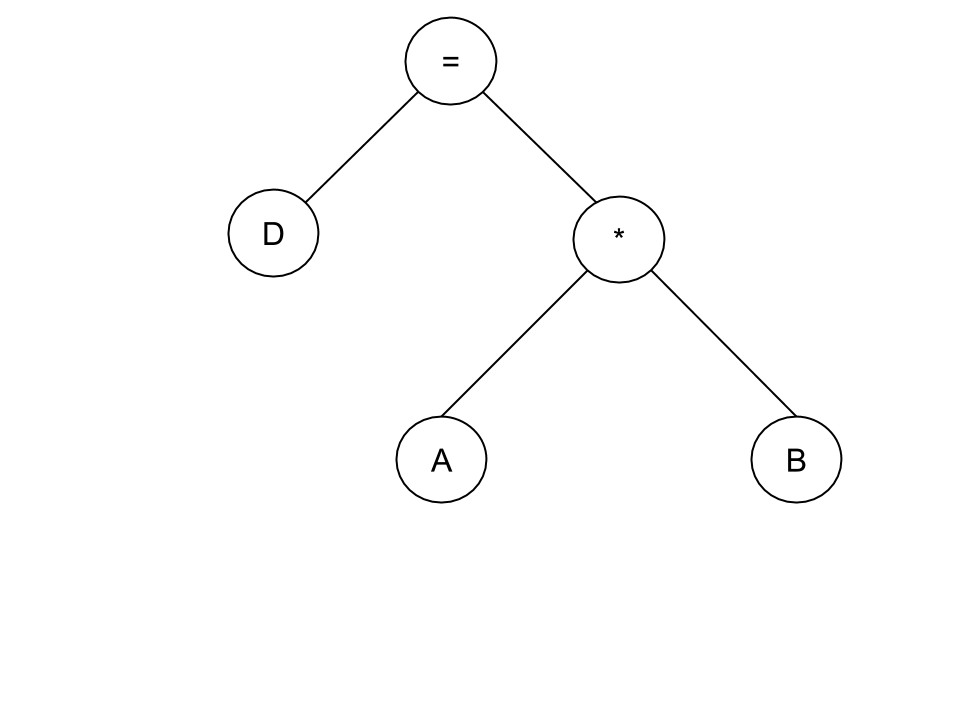
\includegraphics[scale=0.5]{Figures/no_tac.png}
\caption[Statement in \matlab in three address code]{The figure gives an example of an statement in \matlab which is already in three address code and hence is not broken down by Tamer }
\label{Fig:notac}
\end{center}
\end{figure}

In the second case, if the expression is on the LHS, the expression is either a matrix expression or a parameterized expression. In such cases the RHS expression has a temporary variable that is associated with it. The VType for the temporary variable can be generated which will be the VType for the LHS expression. If the expression is on the RHS, the expression itself will have a temporary variable associated with it. \figref{Fig:tac} gives an example of a statement which would be broken down into multiple statements by Tamer. 
\begin{figure}[htbp]
\begin{center}
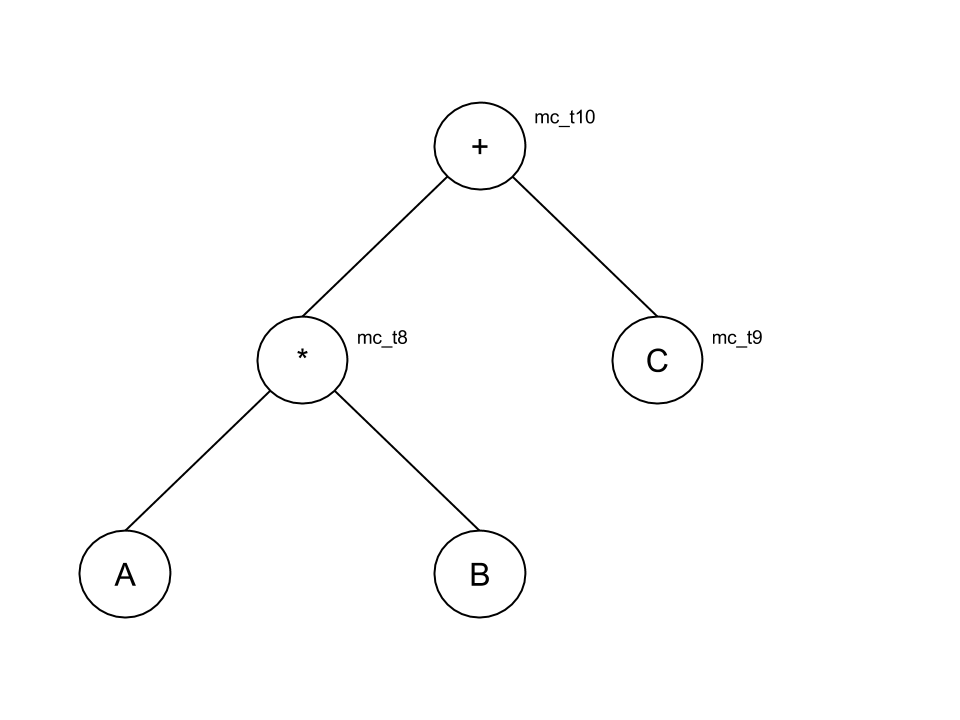
\includegraphics[scale=0.5]{Figures/tac.png}
\caption[Statement in \matlab that is not three address code]{The figure gives an example of an statement in \matlab which is not in three address code and hence is broken down by Tamer using temporaries}
\label{Fig:tac}
\end{center}
\end{figure}
As we can observe each sub-expression has a temporary variable to which it is assigned. The output of the plus expression is assigned to the variable \textsf{mc\_t10} and the output of the multiplication expression is assigned to \textsf{mc\_t8}. The type, shape and whether the expressions are real or complex can be determined by fetching the same information for the temporaries from the analyses. 
\section{Colon Expression transformation}
\label{sec:colonExpr}
The colon expression in \matlab is used in index operations when all the elements of one or more dimensions have to be specified. Listing \ref{lst:colonExprEx} gives an example of an index operation with a colon expression. The second index of the index operation on array A, is a colon expression. The colon expression selects all the columns of the array A. For every column index, the element in row 1 is selected. Thus, the index operation will fetch that all values from all the column that are in the first row. Note that we are assuming that the A is a matrix. If the number of dimensions are greater than 2 (greater than the number of indices), the stop value for the colon expression is the product of all the dimension sizes starting from the second dimension. We call this as array dimension flattening. 
\begin{lstlisting}[language=matlab, label={lst:colonExprEx}, caption={An example of the an array index operation with a colon expression as an index. }]
... = A(1,:);
\end{lstlisting}
In this case, if there are 3 dimensions in total, the stop value of the colon expression will be the product of the sizes of the second and the third dimensions. 

There is no equivalent statement in VRIR. In order to generate a range, we need the start and stop values. The start value will always be one. In order to fetch the stop value, we implemented a transformation which inserts the code to calculate the stop value of the colon expression.This transformation takes into account that an dimensions will have to be flattened if the the colon expression appears as the last index of of the array index operation. 

We insert a statement before the index operation which stores the size of the dimensions for which the colon expression appears. If the colon expression appears as the last index of the array index operation, we also insert a for loop which takes a product of all the dimension sizes starting from the index position where the colon expression appears to the last dimension of the array. The colon expression is then replaced by range expression with the start value as 1 and the stop value as the calculated size. The range expression can then be compiled to the range described in Subsection \ref{subsec:range}. Table \ref{tab:colonExpr} gives an example of how the McSAF IR is transformed. The first column shows the pretty printed McSAF code before the transformation and the second column shows the pretty printed McSAF after the transformation. The code contains three array index operations, each of which have a colon expression. Since for all three index operations the colon expression appears as the last index, a for loop is also inserted which flattens the array dimensions should the number of dimensions be greater than the number of indices. Moreover, the colon expression is replaced by the range expression with the start value as one and the stop value the one which was calculated.
\begin{table}[htbp]
\centering
\begin{tabular}{|l|l|}
\hline

McSAF (Before transformation) & McSAF (After transformation)\\
\hline
{
\begin{lstlisting}[language=matlab,frame=none, numbers=none]
dr(:) = (R(jj,: ) - R(ii, :));
\end{lstlisting}
}
&
{
\begin{lstlisting}[language=matlab,frame=none, numbers=none]
dim_temp4 = 1;
for dim_temp5 = (1 : ndims(dr));
	dim_temp4 = (dim_temp4 * 
				size(dr, dim_temp5));
end;
dim_temp6 = 1;
for dim_temp7 = (2 : ndims(R));
	dim_temp6 = (dim_temp6 * 
				size(R, dim_temp7));
end;
dim_temp8 = 1;
for dim_temp9 = (2 : ndims(R));
	dim_temp8 = (dim_temp8 * 
				size(R, dim_temp9));
end;
dr((1 : dim_temp4)) = (R(jj, (1 : dim_temp6)) - 
					   R(ii, (1 : dim_temp8)));
\end{lstlisting}

}
 \\
\hline
\end{tabular}
\caption[Example of the colon to range expression transformation]{The table gives an example of the transformation from the colon expression to a range expression. }
\label{tab:colonExpr}
\end{table}

\chapter{Generating C++ from VRIR} \label{chap:vrirBackend}
An important contribution of the thesis is the static generation of C++ code from VRIR. Due to differences in the semantics of VRIR and C++, we faced various challenges during code generation. As described in \chapref{chap:Background}, VRIR is a high level strongly typed AST designed to support easy compilation of a wide range of Array based languages. Hence, it supports different indexing schemes such as 0-indexing, 1-indexing and negative indexing as well as different array layout schemes such as row-major and column-major. C++ on the other hand does not have an in-built support for arrays, and only supports 0-indexing and a row major layout. Moreover, VRIR also supports multiple returns. On the other hand, we can only return a single value, which can be a scalar, class, struct or a pointer, in C++. This chapter describes how different nodes in VRIR are mapped to C++ constructs including those which C++ does not implicitly support.
\section{Mapping types}
\subsection{VRIR types}
Data types in VRIR, known as VTypes, can be categorised into 5 types :
\subsection{Scalar type}
The scalar type is used define the primitive data type.
Different types of Scalar values are Int32, Int64, Float32, Float64 and Bool.
The mapping of VTypes to different C++ types is shown in table \ref{tab:typeMap}.
\begin{table}[h]
\centering
\begin{tabular}{|C{3cm}|C{3cm}|}
\hline
VTypes  & C++ types \\ \hline
Int32   & int       \\ \hline
Int64   & long      \\ \hline
Float32 & float     \\ \hline
Float64 & double    \\ \hline
Bool    & bool      \\ \hline
\end{tabular}
\caption[VType to C++ type mapping]{VType to C++ type mapping. The tables shows the different C++ types in the column on the right will be mapped to from the VTypes in the right.} 
\label{tab:typeMap}
\end{table}
\subsection{Array Types}
\section{Operators}
\section{VrArrays}
\section{Statements}
\subsection{Assignment statement}
\subsection{For Statement}
\section{Basic Indexing}
\subsection{ Generating single index value from multiple indices}
\subsection{negative indexing}
\section{Advanced indexing}
\subsection{VrIndex}
\subsection{Array Slicing}

\chapter{Glue Code Generation} \label{chap:glueCode}
The \velocty compiler generates C++ code for functions identified as computationally intensive by the user. The rest of the code is not compiled. Thus, since the computationally intensive functions and the remaining part of the program are in two different programming languages, namely C++ and the source language, an interface between the two code sections is required. Most high-level languages provide an API to interface with C/C++. PyVrir generates the required interface or glue code for Python. However, no glue code generator exists for \matlab.  Hence, along with generating VRIR, we also generate C++ code required to interface \matlab programs with the generated functions. The \matlab MEX API is used for the interface. 
\section{Generating code for including header files}
Header files are required for the following reasons.
\begin{itemize}
\item Declarations of MEX functions. 
\item Declaration of functions in the runtime library. 
\item Declaration of OpenMP functions.
\end{itemize}
The header files are included using the "include" preprocessor directive. 
\begin{lstlisting}[float,language=c,caption={Example of header files in glue code},label={lst:glueCodeHeader}]
#include<mex.h>
#include"matrix_ops.hpp"
#include"library_ops.hpp"
#include"matmul_pImpl.hpp"
#include<omp.h>
\end{lstlisting}
Listing \ref{lst:glueCodeHeader} gives an example of the header files that are generated. The header file "mex.h" provides the set of declarations for the MEX API functions. The header files matrix\_ops.hpp, library\_ops.hpp contain class and function declarations of our runtime library. Function declarations of the generated code are provided by matmul\_pImpl.hpp. The file omp.h is provided for OpenMP functions and directives. 
\section{Generating mexFunction}
The entry point for any shared library that can be called from \matlab is called mexFunction. Listing \ref{lst:mexFunction} gives an example of the mexFunction. The function returns void. It takes four input arguments. The first argument nlhs defines the number of output parameters of the function and the second argument is an array of output parameters. The output parameters are of type mxArray which is a \matlab specific array representation. 
\begin{lstlisting}[language=c,caption={The entry point function for the MEX API},label={lst:mexFunction}]
void mexFunction(int nlhs, mxArray *plhs[],
    int nrhs,const mxArray *prhs[])
\end{lstlisting}
\subsection{Generating VrArrays from mxArrays}
The arrays in the generated functions are represented as VrArrays. VrArrays are a \velocty specific representation of arrays. VrArrays contain the array data as well as meta-data such as the number of dimensions and the dimensions themselves. More information on VrArrays can be found in Subsection \ref{subsec:vrarrays}. VrArrays were used in place of the language specific representation because accessing data and meta-data of mxArrays was expensive. Since the arrays are passed as mxArrays from \matlab and the arrays are represented as VrArrays in the generated code, the glue code has to convert the mxArrays passed as input from \matlab to VrArrays before they can be passed to the generated functions. 

We have implemented methods which convert mxArrays to VrArrays. There is a separate method for each VrArray type. Listing \ref{lst:getVrArray} gives an example of the function used to convert mxArrays to VrArrays. The function is called getVrArrayF64 which takes a pointer to a mxArray as input and returns a VrArrayF64, an array of doubles. Table \ref{tab:getVrArray} gives a list of all the functions for converting VrArrays to different mxArrays. 

\begin{lstlisting}[language=c,caption={Converting mxArrays to VrArrays},label={lst:getVrArray}]
VrArrayF64 y = getVrArrayF64(rhs[1]);
\end{lstlisting}

\begin{table}[htbp]
\centering
\begin{tabular}{|c|c|}
\hline
Function       & Description                         \\ \hhline{|=|=|}
getVrArrayF64  & Returns an array of doubles         \\ \hline
getVrArrayF32  & Returns an array of floats          \\ \hline
getVrArrayCF64 & Returns an array of complex doubles \\ \hline
getVrArrayCF32 & Returns an array of complex floats  \\ \hline
getVrArrayI32  & Returns an array of 32 bit integers \\ \hline
getVrArrayI64  & Returns an array of 64 bit integers  \\ \hline
\end{tabular}
\caption{List of functions used to convert mxArrays to VrArrays.}
\label{tab:getVrArray}
\end{table}

There is an additional overhead while converting from complex mxArrays to complex VrArrays because the representation of the data in the two array types is different. mxArrays store the real and imaginary data as separate arrays. On the other hand, in VrArrays, the real and imaginary data is interleaved. Thus, for every element of the array, the real value is immediately followed by the imaginary value.

Scalar values are also passed as mxArrays by \matlab where as they are represented using the C++ primitive types. The glue code also converts the mxArrays to scalar types when required. Listing \ref{lst:getScalar} gives an example of the conversion. The example shows a mxArray pointer rhs[5] being converted to a scalar value inputData5. The MEX function, mxGetScalar returns a scalar double value. A cast is required for all types other than double.
\begin{lstlisting}[language=c,caption={Converting mxArrays to scalars},label={lst:getScalar}]
 double inputData5 = static_cast<double>(mxGetScalar(rhs[5]));
\end{lstlisting}

\subsection{Function Call}
Once all the input parameters are converted to VrArrays or C++ primitive types, we make a call to the generated entry point function. The output of the function is stored in either a VrArray or a scalar variable if the function returns a single variable. Listing \ref{lst:funcCall} gives an example of the generated function call. The listing shows a call to the function babai which returns a VrArrayF64 which is assigned to the variable retVal.
\begin{lstlisting}[language=c,caption={Call to generated function},label={lst:funcCall}]
VrArrayF64 retVal = babai(R,y);
\end{lstlisting}

The generated function can also return multiple variables of different types. In this case the generated function packages the  variables into a struct and returns the struct. More information about multiple returns can be found in Subsection \ref{subsec:multreturn}. Listing \ref{lst:funcCallMult} gives an example of a call to a function with multiple returns. The function name is nb1d which takes 7 inputs and returns a struct of type struct\_nbody1d\_ret retVal.
\begin{lstlisting}[language=c,caption={Call to generated function},label={lst:funcCallMult}]
struct_nbody1d_ret retVal = nbody1d(inputData0,inputData1,
							inputData2,inputData3,
							inputData4,inputData5,inputData6);
\end{lstlisting}
\subsection{Converting to mxArrays}
The output of the generated function has to be returned to \matlab. The output can consist of a single or multiple variables. The output can be returned via the array plhs. As mentioned earlier, plhs is an array of mxArray pointers. Hence the output of the generated function, which is either a VrArray or a C++ primitive type has to be converted to mxArrays and stored as successive plhs elements. We use MEX API functions to do the same. 

In case of VrArrays, we first have to create an array of the required size. We do this using the function mxCreateNumericArray. This function takes as input, the number of dimensions, an array of dimension sizes, the data type of the array and its complexity. We use the ndims and dims fields from the VrArray to specify the number of dimensions and the sizes of each dimensions. Once the array is created, we set the mxArray data by passing the pointer to the data inside the VrArray to the the function mxSetData.

For scalar values, we use the MEX function mxCreateNumericMatrix which accepts the row and column sizes as well as the complexity and  the type of the array.We set the row and column sizes as one. We then fetch a pointer to the data of the newly created mxArray and set the zero$^{th}$ element to the scalar value. 

If the function returns multiple output values, each data member of the return struct is used to create an mxArray which is then assigned to successive indices of plhs. 

\chapter{Code Optimisations} \label{chap:codeOptimise}
The primary goal of the thesis was to ensure correct compilation of code from \matlab and Python to C++. An additional goal was to improve the performance of the generated code. Initial experiments showed that turning on bounds check slowed down 6 of the 17 benchmarks and 3 of the 9 benchmarks in Python. The geometric mean of the slowdown compared to bounds check turned off was 3.66 for \matlab and 1.63 for Python. Additionally, while analysing the generated code, we found that array operations being performed inside loops were allocating memory to the same output array for every iteration. We determined that by optimising the code to eliminate bounds checks and unnecessary memory allocations, we gain a significant improvement in performance. In this chapter we first discuss the bounds check implementation followed by the two optimisations, namely elimination of bounds checks and elimination of redundant memory allocations. 

\section{Bounds Checks}
Scientific languages like \matlab and Python support array bounds checks for indexing operations. These checks ensure that the program does not crash abruptly and instead throws an error before exiting. On the other hand, C++ does not implicitly support array bounds checks. Hence we provide bounds checks through the runtime library.

Due to differences in semantics of \matlab and Python, the bounds check implementations for both languages are different. Hence we provide different implementations for the two languages. Array growth is also carried out by the bounds check implmentation for languages that support it. 

However, the API for both language implementations is the same. The entry point function for bounds checks is a templated function called \textsf{checkBounds}. Listing \ref{lst:boundscheck} gives an example of the bounds check function for the array \textsf{c}. The bounds check functions are called inside conditional blocks which allows the user to turn the checks on or off while compiling the code. The first parameter is the reference to array on which the indexing operation is performed. The second parameter is a boolean flag which is set to true if the boolean operation is on the LHS of an assignment statement. This flag is used to determine if the array should be grown when one or more indices exceed bounds. This check is only used by the \matlab implementation. The third parameter is the number of indices. This parameter is required since the function accepts variable arguments. The remaining parameters are the indices which are passed as VrIndex structs. Passing indices as VrIndex structs allows the function to handle different index types such as ranges and arrays.

\begin{lstlisting}[language=c,caption={An example of the bounds check function call.},label={lst:boundscheck}]
//Bounds check 
#ifdef BOUND_CHECK
	checkBounds<VrArrayPtrF64,double>(&c,false,2,vrIndex(i),vrIndex(j));
#endif
\end{lstlisting}


However, the default bounds check function performs poorly due to dynamic memory allocation. The implementation inserts the indices into an array and performs checks while iterating over the array. Using an array simplifies the code for the checks. However, since the number of indices can vary, the array cannot be created at compile time.

In order to improve performance of the bounds checks, we implemented specialised versions of the bounds check function for index operations with one, two and three indices. We also implemented three additional versions for index operations where all indices have numeric values. These specialised functions are called checkBounds\_spec. Listing \ref{lst:boundscheck_spec} shows an example of the specialised version of the bounds check function. The function is specialised for two indices, both of which have numeric values. The first two parameters denote the array and whether the operation is performed on the LHS like in the default function. The remaining two parameters are the indices. 
\begin{lstlisting}[float,language=c,caption={An example of the specialised bounds check function call},label={lst:boundscheck_spec}]
//Bounds check 
#ifdef BOUND_CHECK
	checkBounds_spec<VrArrayPtrF64,double>(&c,false,
		static_cast<dim_type>(i),static_cast<dim_type>(j));
#endif
\end{lstlisting}
\section{Bounds Check Elimination}
Slowdown when the bounds checks was identified to be higher when the checks are performed inside loop bodies. In such cases, the checks are performed for every loop iteration resulting in the slowdown. Consider the example given in Listing \ref{lst:example_optim}. The example contains an index expression on the array y inside a loop. The index expression consists of a single index (k-1). The loop has a starting value of 1 and a final value of n-1. The value of the loop variable k is incremented by one with every iteration. As we can see, the index is a linear function of the loop variable k. The loop bounds are not modified inside the loop. Moreover, the step value of the loop is a constant and hence it can be inferred that the loop direction is upwards, that is, the loop iterates from a smaller start value to a larger stop value. By replacing the loop variable by the start and stop expressions of the loop, we get the lower and upper bounds of the index respectively. Thus the smallest value of the index inside the loop will be (1-1), that is, 0 and the largest value of the index will be ((n-1) - 1), that is, (n-2). Since we know what the lower and upper bound of the index, we can check whether these values exceed the array size or are less than the lowest index value supported by indexing scheme, outside the loop. If the index is valid, the there is no need to perform bounds checks inside the loop. Thus this technique would improve the performance of the program. We use this optimisation technique, on a subset of the indices known as affine indices. 
\begin{lstlisting}[float,language=c,caption={Example C++ for loop with array index expressions},label={lst:example_optim}]
   for(k=1;k<=(n-1);k=k+1)
       {
  #ifdef BOUND_CHECK
          checkBounds_spec<VrArrayPtrF64,double>(&y,false,
				static_cast<dim_type>(k-1));
  #endif
          vr_temp12 = VR_GET_DATA_F64(y)[(k - 1)];
      }
\end{lstlisting}
\subsection{Affine indices}
A function of one or more variables is considered to be affine if it can be expressed as a sum of constant and constant multiples of the variables. Equation \ref{eq:affineIndex} gives a mathematical representation of affine functions. 
\begin{equation}
\label{eq:affineIndex}
f = C_0 + \sum\limits_{i=1}^n C_iX_i 
\end{equation}
where $C_i$ is the $i^{th}$ constant and $X_i$ is the $i^{th}$ variable. 

Affine indices can be defined as array indices which are affine functions of the loop induction variables. Table \ref{tab:affineIndex} gives examples of affine and non-affine array indices. 
\begin{table}[htbp]
\centering
\begin{tabular}{|c|c|}
\hline
Array Index & Affine \\ \hhline{|=|=|}
A(2*i+1)    & Yes    \\ \hline
A(i-1)    & Yes    \\ \hline
A(i*j)      & No    \\ \hline
A(i*i)      & No     \\ \hline
A(b(i))     & No     \\ \hline
\end{tabular}
\caption{Examples of affine and non-affine indices}
\label{tab:affineIndex}
\end{table}
\subsection{Technique}

The process of moving the checks outside the loop body can be divided into two parts. Identifying index operations which can be moved outside the loop and generating a if condition for the checks and two versions of the loop body.   

\subsubsection{Identifying valid index operations}
We define valid index operations to have the following properties. 
\begin{enumerate}
\item All indices should be affine functions of the loop variables. 
\item All the loop variables should have loop invariant bounds. 
\end{enumerate}
In order to determine whether a check for an index operation can be moved outside the loop body, we check whether individual indices are affine. Indices in VRIR are represented by IndexStructs. We do not consider indices which are ranges or expressions with non-scalar types. For indices withs scalar expressions, we recursively traverse the expression until we reach a name or a constant expression or we reach an unsupported expression. Constant expressions are considered affine. In  case of name expressions we check whether the expression is a loop invariant or a loop variable. If the expression is a loop variable, we check whether the loop bounds are loop invariant. Apart from constant and name expressions, we also support binary and unary expressions. We only support a specialised case of the mult expression where the LHS and RHS  of the expression are either name or constant expressions. If both the LHS and the RHS are name expressions, they should both not be loop variables. We support the same expressions for checking the validity of loop bounds. The set of supported expressions are given in Table \ref{tab:affineIndexCheck}. 
\begin{table}[htbp]
\centering
\begin{tabular}{|c|c|}
\hline
Expression Name & Description        \\ \hhline{|=|=|}
plus            & Scalar Addition    \\ \hline
minus           & Scalar Subtraction \\ \hline
name            & Variable Name      \\ \hline
negate          & Unary Minus        \\ \hline
const           & Constant Value     \\ \hline
\end{tabular}
\caption{List of supported expressions for affine index check}
\label{tab:affineIndexCheck}
\end{table} 
\subsubsection{Generating code}
To implement the optimisation, the compiler generates an if statement. The if condition contains the checks for the valid index operations. For every index operation, we perform two checks. One for the lower bounds and another for the upper bounds. These checks are performed through functions called checkDimStart for the lower bounds and checkDimStop for the upper bounds. The functions takes as input integer indices. VrIndex structs are not required since indices containing ranges or having non-scalar types are not considered to be valid by the analysis. These functions are implemented inside the runtime library. The specialised functions for one two and three indices are also implemented in the library. Listing \ref{lst:boundsoptim} gives an example of the default and specialised functions. The default functions take the array name, the number of indices and the indices as parameters. The specialised functions named <default function name>\_spec take the array name and the indices as parameters. In the example, the functions take 2 indices as input. The loop variables are replaced by the lower and upper bounds of the loops when being passed as arguments to the check functions.We use the loop direction to determine whether the loop variables need to be replaced by the lower bounds for checkDimStart and upper bounds for checkDimStop or vice versa. If loop direction is up, that is the lower bound value is smaller than the upper bound value, the lower bound are used in checkDimStart and upper bound for checkDimStop. 

Listing \ref{lst:boundsoptimBlock} gives an example of the if statement generated by the compiler. The example shows a total of 6 functions, three for the lower bounds and three for the upper bounds of three arrays A, B and c. If the checks return true, a checks free version of the code is executed else the default version with checks is turned on is executed. 
\begin{lstlisting}[float,language=c,caption={An example of the default and specialised function calls for the boundscheck optimisations},label={lst:boundsoptim}]
//Default function
checkDimStart<VrArrayPtrF64>(c,2,1,1)
checkDimStop<VrArrayPtrF64>(c,2,m,n)

//Specialised function
checkDimStart_spec<VrArrayPtrF64>(c,1,1)
checkDimStop_spec<VrArrayPtrF64>(c,m,n)
\end{lstlisting}
\begin{lstlisting}[float,language=c,caption={An example of the if statement generated for the boundscheck optimisations},label={lst:boundsoptimBlock}]
 if(checkDimStart_spec<VrArrayPtrF64>(c,1,1) && checkDimStop_spec<VrArrayPtrF64>(c,m,n) && 
		checkDimStart_spec<VrArrayPtrF64>(B,1,1) && checkDimStop_spec<VrArrayPtrF64>(B,k,n) && 
		checkDimStart_spec<VrArrayPtrF64>(A,1,1) && checkDimStop_spec<VrArrayPtrF64>(A,m,k)) {
			<For Statements without bounds check >	
		} else {
			<For Statements with bounds check >	
		}
	
\end{lstlisting}
\section{Eliminating unnecessary memory allocations}
\label{sec:memoptimise}
Array operations and array slicing are implemented through functions in the runtime library. The output of these operations is written to a new array created inside the functions. Many times these operations are performed inside loops and the output is assigned to the same array variable. However, runtime memory allocation in expensive. Consider the example in Listing \ref{lst:memOptimiseExample}. The example contains an array operation, scal\_minus, which subracts a scalar vr\_temp28  from every element in the array Rx and assigns it to an array that is created inside the function. The output of this operation is assigned to another array drx. Since this function is called inside the loop, a new array would be created on every loop iteration. However output array that is created will always be assigned to drx. The number of memory allocations could be reduced by reusing the memory that was assigned to drx during the first iteration for the subsequent iterations. Memory can only be reused if the size of drx is greater than or equal to the output of scal\_minus. Hence, the functions will have to be modified to perform a check for ensuring memory can be reused. Moreover, the function signature will have to to be modified to add a reference to the array to which the output is assigned, in this case, drx. Another alternative and is to implement a specialised function for the optimisation which satisfies the above mentioned criterion. We chose the second alternative for the optimisation. 
\begin{lstlisting}[float,language=c,caption={An example of an array operation which is optimised },label={lst:memOptimiseExample}]
for(k=1;k<= n;k=k+static_cast<long>(1)) {
	drx = BlasDouble::scal_minus(Rx,vr_temp28);
}
\end{lstlisting}

\subsection{Supported Functions}
Since a check for sufficient memory allocation needs to be made inside the function, a reference to the output array also needs to the be passed. Hence we implement specialised functions for this optimisation. The Supported library functions include many of the  array operations described in Subsection \ref{subsec:arrayOps} and a few other library functions. For dimension collapsing functions we support cases where a scalar value is returned. Table \ref{tab:memoptimiselist} gives a list of functions for which an implementation support the memory optimisation exists. 
\begin{table}[htbp]
\centering
\begin{tabular}{|c|c|c|}
\hline
Function Name & Function description         & Scalar version \\ \hhline{|=|=|=|}
mmult         & Matrix multiplication        & Yes            \\ \hline
scal\_mult    & Scalar Matrix Multiplication & No             \\ \hline
vec\_add      & Array Addition              & No             \\ \hline
vec\_copy     & Array Copy                   & No             \\ \hline
vec\_sub      & Array Subtraction            & No             \\ \hline
scal\_add     & Scalar Array Addition        & No             \\ \hline
scal\_minus   & Scalar Array Subtraction     & No             \\ \hline
transpose     & Matrix Transpose             & No             \\ \hline
sum           & Sum of Array Elements        & Yes            \\ \hline
mean          & Mean of Array Elements       & Yes            \\ \hline
sliceArray          & Get array slice        & No            \\ \hline
\end{tabular}
\caption{List of functions that support memory optimisation}
\label{tab:memoptimiselist}
\end{table}
\subsection{Checking for Sufficient Memory}
As mentioned before, the specialised functions accept a reference to the output array as an input parameter. The output array is then checked to determine whether the maximum number of elements that the array can hold is greater than or equal to the number of elements of the output of the operation performed by the function. The number of elements are calculated by taking the product of the dimensions of the array. If the memory is sufficient, no memory is allocated to the array whereas memory is allocated if it is not sufficient. In either case, the dimensions are modified to be equal to the expected dimensions of the output of the array operation.   
\subsection{Code Generation}

\begin{table}
  \begin{tabular}{|l|l|}
  \hline
  Array operation without optimisation & 
Array operation with optmisation 
   \\
  \hhline{|=|=|}
  
  {
  \begin{lstlisting}[language=c,frame=none, numbers=none]
	drz = 
		BlasDouble::scal_minus(Rz, vr_temp30);
  \end{lstlisting}
  } &
   {
   \begin{lstlisting}[language=c,frame=none, numbers=none]
	 BlasDouble::scal_minus(Rz, 
		vr_temp30,&drz);
   \end{lstlisting}
   } \\
   \hline
   \end{tabular}
   \caption[Generated code with and without memory optimisations]{Table shows the generated code with and without memory optimisations}
   \label{tab:memOptimise}
   \end{table}
While generating code for assignment statements, the compiler checks for library call expressions which can be compiled to specialised function calls. The compiler does this by checking the function name against a hash set which stores a list of functions that can be specialised. The compiler generates the specialised function call in place of the assignment statement. It then passes the reference LHS of the assignment statement as a parameter to the function. 

Table \ref{tab:memOptimise} gives an example of the generated codes with and without the memory optmisations. The left column shows the function call without the optimisation and the right column shows the function call with the optimisation. The example shows an array operation scal\_minus which subtracts a scalar vr\_temp30 from every element in the array Rz and assigns the result to drz. The optimisation passes the output array drz's reference to the function where a check for sufficient memory is performed.

\chapter{Results} \label{chap:results}
A major goal of the thesis was to improve the performance of array-based languages like \matlab and Python's NumPy library by compiling computationally intensive functions to C++. To demonstrate these performance results, we compared the performance of the generated code with that provided by various tools for scientific computing. Seventeen \matlab benchmarks and nine Python benchmarks were used to perform this comparision. Different variations of generated code that can be generated by turning optimisations on and off were also tested. 

In this chapter, we give a brief description of the benchmarks that were used to test the performance followed by the results themselves and our analysis of these results. 
\section{Benchmarks}
Two separate set of benchmarks  were used for \matlab and Python. 
\subsection{\matlab Benchmarks}
The \matlab benchmarks used for the performance were obtained from various sources. The sources include the FALCON project\cite{DeRose:1999} , the OTTER project \cite{quinn}, Chalmers university of technology\footnote{\url{http://www.elmagn.chalmers.se/courses/CEM/}}, Mathworks central file exchange\footnote{\url{http://www.mathworks.com/matlabcentral/fileexchange}} and the presentation on parallel programming in \matlab by Burkhadt and Cliff\footnote{\url{http://people.sc.fsu.edu/~jburkardt/presentations/matlab_parallel.pdf}}. The benchmarks cover commonly occurring \matlab features such as builtin function calls, array indexing including slicing operations and array operations like array addition, matrix multiplication, etc. Table \ref{tab:matBench} gives the list of benchmarks used along with their descriptions and source.  
\begin{table}[htbp]
\resizebox{\columnwidth}{!}{%
\centering
\begin{tabular}{|c|c|c|}
\hline
Benchmark  & Source               & Description\\
\hhline{|=|=|=|}
bbai       & MATLAB file exchange & Implementation of the Babai estimation algorithm \\
\hline 
bubble       & McLab                & Bubble Sort \\
\hline 
capr       & Chalmers University  & \begin{tabular}{@{} c@{}} Computes the capacitance of a transmission line \\ using fine difference and Gauss-seidel\end{tabular} \\
\hline 
clos       & Otter project        & Calculates the transitive closure of a directed graph \\
\hline 
crni       & Falcon project       & Crank-Nicholson solution to the heat equation \\
\hline
dich       & Falcon project       & Dirichlet solution to Laplace's equation\\
\hline
fiff       & Falcon project       & Computes the finite difference solution to the wave equation \\
\hline
ldgr       &  -                    & Calculates derivatives of Legendre polynomials \\
\hline
mbrt       & McFor project        & Computes Mandelbrot sets \\
\hline
nb1d       & Otter project        & Simulates the 1-dimensional n-body problem \\
\hline
matmul     & McLab                & naive matrix multiplication \\
\hline
mcpi       & McLab                & Calculates $\pi$ by the Monte Carlo method   \\
\hline
numprime   & Burkardt and Cliff   & \begin{tabular}{@{} c@{}} Simulates the sieve of Eratosthenes for  \\calculating number of prime numbers less than a given number \end{tabular} \\
\hline
scra       & ACM CALGO            & \begin{tabular}{@{} c@{}} Implementation to produce a reduced-rank \\ approximation to a matrix \end{tabular}   \\
\hline
spqr       & ACM CALGO            & \begin{tabular}{@{} c@{}} Implementation to compute a pivoted \\ semi-QR decomposition of an m-by-n matrix A \end{tabular} \\
\hline
quadrature & Burkardt and Cliff   &  \begin{tabular}{@{} c@{}} Simulates the quadrature approach \\ for  calculating integral of a function \end{tabular} \\
\hline
\end{tabular}
}
\caption[List of \matlab Benchmarks]{List of \matlab Benchmarks used for experiments}
\label{tab:matBench}
\end{table}
\subsection{Python Benchmarks}
Many of the Python benchmarks are Python ports of the Ostrich benchmark suite\cite{Khan:2014:UJW:2661088.2661090}. The benchmarks contain scalar operations as well as array index operation. Six of the nine Python benchmarks support parallelism. Table \ref{tab:pyBenches} gives the list of Python benchmarks that were used. The Python ports of the Ostrich benchmark suite are known as PyDwarfs. The rest of the benchmarks are part of a suite that were put together by the open-source Python community focused on compilers. The suite is known as NumFocus and can be found  on github\footnote{\url{https://github.com/numfocus/python-benchmarks}}. 
\begin{table}[htbp]
\centering
\begin{tabular}{|c|l|c|}
\hline
Benchmark Name & Source    & Description                                                                                                                                              \\ 
\hhline{|=|=|=|}
arc\_distance  & NumFocus & \begin{tabular}[c]{@{}c@{}} Calculates the pairwise arc distance \\ between all points in vector a and b.\end{tabular} \\ \hline                                                                                                                                                   
fft            & Pydwarfs  & Fast Fourier Transform                                                                                                                                   \\ \hline
growcut        & NumFocus &  Implementation of GrowCut segmentation                                                                                                                                                         \\ \hline
julia          & NumFocus &  Calculates the Julia fractal                                                                                                                                                        \\ \hline
lud            & PyDwarfs  & \begin{tabular}[c]{@{}c@{}}LU decomposition  factors a matrix as the product of a \\ lower triangular matrix and an upper triangular matrix\end{tabular} \\ \hline
pagerank       & PyDwarfs  & PageRank is a link analysis algorithm used by Google Search                                                                                              \\ \hline
pairwise       & NumFocus &   \begin{tabular}[c]{@{}c@{}} Computes the pairwise distance \\ between a set of points in 3D space.\end{tabular}                                                                                                                                                         \\ \hline
spmv           & PyDwarfs  & Sparse Matrix-Vector Multiplication                                                                                                                      \\ \hline
srad           & PyDwarfs  & \begin{tabular}[c]{@{}c@{}}Tracks the movement of a mouse heart over a sequence  of 104\\ 609x590 ultrasound images to record response to the stimulus \end{tabular} 
\\ \hline
\end{tabular}
\caption[List of Python Benchmarks used for experiments]{List of Python Benchmarks used for experiments}
\label{tab:pyBenches}
\end{table}

\section{Experimental Setup}
We ran separate experiments for \matlab and Python benchmarks. Different variations of the code generated by \velocty were also tested. Table \ref{tab:benchvar} gives a list of variations generated by \velocty. All the benchmarks were tested on a machine running GNU/Linux(3.8.0-35-generic \#52-Ubuntu) with a Intel(R) Core(TM) i7-3820 CPU @ 3.60GHz with 16GB of memory. We also ran experiments on different compiler tools developed for both \matlab and Python. Each version of the benchmarks was executed 10 times and the average execution time was recorded. The following subsections describe the tools for each language against which the different versions of \velocty were compared and explain the aspects of the experimental setup that are specific to each language.

\begin{table}[h]
\centering
\begin{tabular}{|c|c|}
\hline
Variation name                                                               & Description                                                                                                                        \\ \hhline{|=|=|}
Baseline VeloCty                                                             & \begin{tabular}[c]{@{}c@{}}Generated C++ code without optimisations and \\ with array bounds checks enabled\end{tabular}           \\ \hline
VeloCty no-checks                                                            & \begin{tabular}[c]{@{}c@{}}Generated C++ code without optimisations and \\ without array bounds checks.\end{tabular}               \\ \hline
VeloCty memory optimisation                                                  & \begin{tabular}[c]{@{}c@{}}Generated C++ code with memory optimisations and \\ with array bounds checks enabled.\end{tabular}      \\ \hline
\begin{tabular}[c]{@{}c@{}}VeloCty bounds check \\ optimisation\end{tabular} & \begin{tabular}[c]{@{}c@{}}Generated C++ code with boundscheck optimisations \\ and with array bounds checks enabled.\end{tabular} \\ \hline
VeloCty parallel                                                             & \begin{tabular}[c]{@{}c@{}}Generated C++ code with parallel constructs \\ and with array bounds checks enabled.\end{tabular}       \\ \hline
VeloCty all optimisations                                                    & \begin{tabular}[c]{@{}c@{}}Generated C++ code with all optimisations\\  and with array bounds checks enabled.\end{tabular}         \\ \hline
\end{tabular}
\caption[List of benchmark variations generated by \velocty]{ The table gives a list of benchmark variations generated by \velocty along with the description of each}
\label{tab:benchvar}
\end{table}

\subsection{Experimental Setup for \matlab}
 In order to gauge \velocty's performance against current compiler tools for \matlab, the \matlab benchmarks were executed on the Mathworks' 2014b release of the \matlab interpreter and JIT compiler. We also used the Mathworks' \matlab-Coder implementation to compile the benchmarks to C++. This generated C++ code is compiled as  a dynamic library similar to the method used by \velocty. Both \velocty and \matlab-coder use the MEX compiler to compile the C++ code and generate the shared library. MEX internally uses the g++-4.6.4 compiler. 
\subsection{Experimental Setup for Python}
 Similar to \matlab, we gauged our performance of the \velocty code against exising compiler tools for Python. We used the reference C-Python interpreter version 3.2.3  and Cython\cite{cython} version 0.21, which is a compiler used to generate C-extensions for Python. Both, \velocty and Cython use g++-4.6.4 through distutils for compilation. 

\section{\matlab Results}

\subsection{Overall Results}
We ran experiments on 17 \matlab benchmarks. We compared the VeloCty with all optimisations enabled  with the Mathworks' \matlab implementation and \matlab-coder. We measured the speedup of the VeloCty backend and the \matlab-coder versions compared to Mathwork's \matlab JIT compiler. Figure \ref{fig:results_cwochecks} shows a bar graph with the results of the experiment. The red bars show the speedup of \matlab-coder and the blue bars show the speedup of the VeloCty backend with all optimisations enabled. The geometric mean for the speedup of the VeloCty version was 8.05x as compared to the geometric mean of 3.89x for the \matlab-coder version. The largest speedup was shown by the quadrature benchmark. The benchmark was 458x times faster than Mathworks' \matlab. The benchmark consists of operations on scalar operations and hence gives a high speedup. The smallest speedup of 1.31x, is given by the closure benchmark. The benchmark's computationally intensive code section is a while loop containing a matrix multiplication operation. All three versions, the VeloCty backend, Mathwork's \matlab and \matlab-coder use the Intel MKL BLAS library and hence show similiar performance. 

\begin{figure}[htbp]
\centering
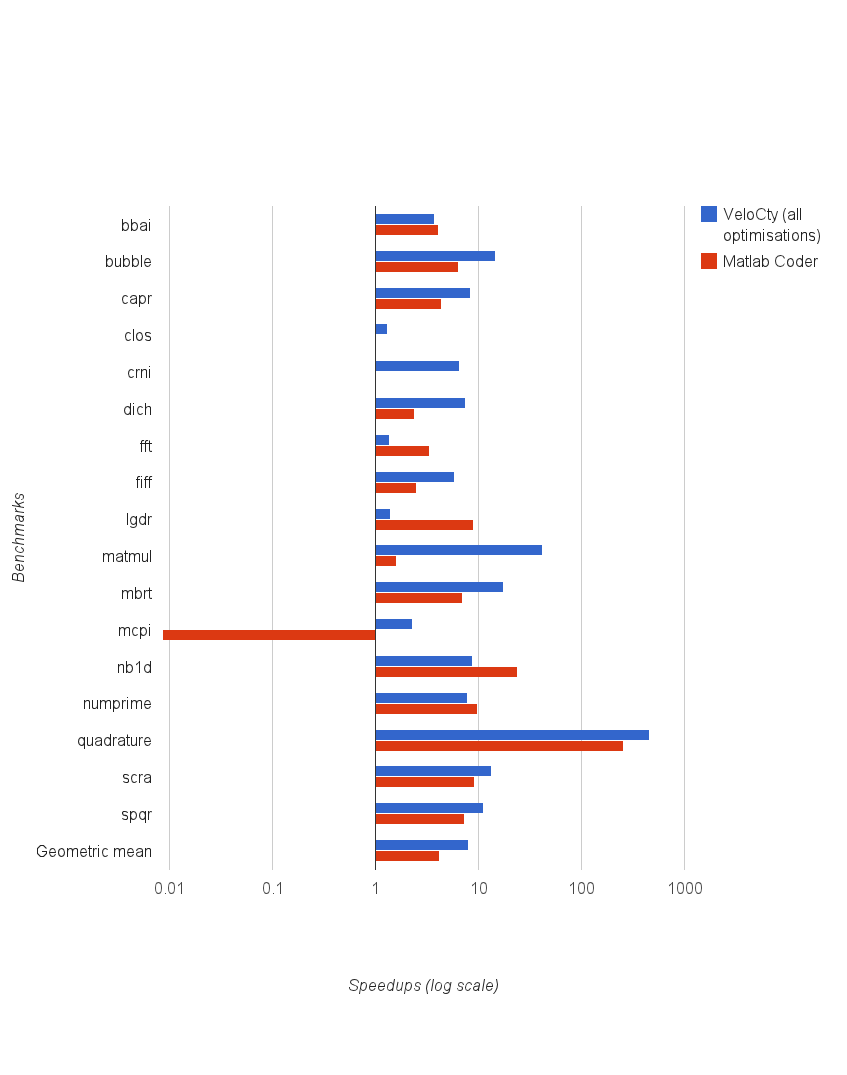
\includegraphics[scale=0.5]{Figures/results_cwochecks.png}
\caption[Experiment results for the baseline \velocty backend for \matlab benchmarks]{The bar graph gives the speedups of the \velocty backend with all optimisations enabled and \matlab-coder compared to the Mathworks' JIT and VM implemenation. Higher is better }
\label{fig:results_cwochecks}
\end{figure}

For most benchmarks, our VeloCty backend was faster than \matlab-coder. The benchmarks, \textsf{bbai}, \textsf{lgdr}, \textsf{nb1d}, \textsf{fft} and \textsf{numprime} are exceptions. \textsf{Lgdr} \textsf{bbai} and \textsf{nb1d} contain array slicing and array operations which do not internally make calls to the BLAS library and hence take longer to execute compared to \matlab-coder. The \textsf{fft} benchmark contains a loop whose direction can not be identified at run time and hence a loop vector needs to be initialised and iterated over as described in Subsection \ref{subsec:forStmt}. \textsf{numprime} contains scalar operations and a square root function call. The square root function's \matlab implementation may be faster than the standard C++ implementation and hence the \textsf{numprime} benchmark performs in \matlab-coder than in the \velocty version. 

As we can also observe, \matlab-coder shows a positive speedup on all benchmarks except for \textsf{mcpi}. The reason for this is that the benchmark contains a loop with calls to the random function inside the body. These functions return a single scalar value. However, in case of \matlab-coder, an 1x1 matrix is returned. Since a heap allocation is needed for every iteration, the benchmark is significantly slower than Mathworks' \matlab. 

The \textsf{crni} benchmark is an example of a feature that is supported by \velocty but not by \matlab-coder. The benchmark contains a growing array which is not supported by \matlab-coder. Hence, a \matlab-coder version of the benchmark cannot be generated. 

\subsection{Impact of Array Bounds Checks on Performance}
Table \ref{tab:CwovsCw} gives the slowdown of the generated VeloCty code because of bounds checks. This experiment allowed us to determine the effect bounds check had on performance. The table lists the slowdown of the baseline \velocty code compared to the \velocty code with checks disabled. 6 benchmarks show a slowdown of 1.5x or higher. These benchmarks are \textsf{bubble}, \textsf{capr}, \textsf{dich}, \textsf{fft}, \textsf{fiff} and \textsf{matmul}. The geometric mean of the slowdown for all benchmarks is 1.66x. If only the geometric mean of the  6 benchmarks that slowed down significantly  are considered, we get a geometric mean of 3.66x. The matmul benchmark shows the highest slowdown with 10.44x. The slowdown for the \textsf{crni} benchmark cannot be calculated since a version of the generated code without checks cannot be executed. 

\begin{table}[htbp]
\centering
\begin{tabular}{|c|c|}
\hline
Benchmarks                           & Slowdown     \\ \hhline{|=|=|}
bbai                                 & 1.21  \\ \hline
bubble                               & 8.61  \\ \hline
capr                                 & 2.62   \\ \hline
clos                                 & 0.84 \\ \hline
crni                                 & -            \\ \hline
dich                                 & 1.71\\ \hline
fft                                  & 1.43\\ \hline
fiff                                 & 4.15\\ \hline
lgdr                                 & 1.01\\ \hline
matmul                               & 10.44\\ \hline
mbrt                                 & 1.02\\ \hline
mcpi                                 & 1.00\\ \hline
nb1d                                 & 1.05\\ \hline
numprime                             & 1.06\\ \hline
quadrature                           & 1.00\\ \hline
scra                                 & 1.99\\ \hline
spqr                                 & 1.04\\ \hline
Geometric mean                       & 1.66\\ \hline
Geometric mean (Affected Benchmarks) & 3.66\\ \hline
\end{tabular}
\caption[Slowdown of \velocty with checks enabled]{The table lists the slowdowns of the  VeloCty baseline code  compared to when \velocty-no-checks}
\label{tab:CwovsCw}
\end{table}
\subsection{Impact of Bounds Check Optimisations on Performance}
The previous experiment showed us that bounds checks have a significant impact on performance. This was the reason we implemented an optmisation to elminate the bounds checks where possible. In order to determine the improvement in performance when bounds check optimisations were enabled, we compared the speedup of the generated VeloCty code with bounds check optimisation enabled  against the baseline \velocty version. Table \ref{tab:CwvsCbc} gives the speedups for all the benchmarks. The geometric mean of speedups with the optimisation enabled is 1.62x. If the speedups of the benchmarks that show a significant speedup are considered, we see a speedup of 3.18x. The \textsf{fft} benchmark does not show an improvement in performance. This is because the benchmark contains a loop whose direction can not be determined and hence the bounds checks inside the loop body  can not be moved outside.
\begin{table}[h]
\centering
\begin{tabular}{|c|c|}
\hline
Benchmarks     & Speedups \\ \hhline{|=|=|}
bbai           & 1.07     \\ \hline
bubble         & 7.84     \\ \hline
capr           & 2.49     \\ \hline
clos           & 1.00     \\ \hline
crni           & 2.23     \\ \hline
dich           & 1.71     \\ \hline
fft            & 1.01     \\ \hline
fiff           & 4.12     \\ \hline
lgdr           & 1.02     \\ \hline
matmul         & 10.54    \\ \hline
mbrt           & 1.00     \\ \hline
mcpi           & 1.00     \\ \hline
nb1d           & 1.06     \\ \hline
numprime       & 0.99     \\ \hline
quadrature     & 1.00     \\ \hline
scra           & 1.04     \\ \hline
spqr           & 1.01     \\ \hline
Geometric mean & 1.62     \\ \hline
\end{tabular}
\caption[Speedup of \velocty with bounds check optimisation turned on]{The table lists the speedups obtained when the array bounds check optimisations are turned on against the baseline \velocty code}
\label{tab:CwvsCbc}
\end{table}
\subsection{Impact of Memory Optimisations on Performance}
As we had already identified that many of the benchmarks contain array operations inside a loop where memory is allocated continuously. As dynamic memory allocations are expensive, we implemented an optmisation to eliminate unecessary memory allocations and instead reuse previously allocated memory where possible. The performance improvement of the generated code when the memory optimisations were enabled was also gauged. We calculated the speedups of the generated VeloCty code with memory optimisations enabled compared to the baseline VeloCty code for all the benchmarks. Table \ref{tab:cmvscwo} gives the speedups for the benchmarks. The geometric mean of the speedups for all benchmarks is 1.14x. Four benchmarks, \textsf{capr}, \textsf{nb1d}, \textsf{scra}, \textsf{spqr} showed speedups of 1.54x, 1.59x, 3.57x and 2.77x respectively. All of these benchmarks consisted of loops inside which array operations were performed. Since, because of the optimisation, previously allocated memory was reused, we observed a noticeable speedup. The geometric mean of the four affected benchmarks is 2.36x. 
\begin{table}[h]
\centering
\begin{tabular}{|c|c|}
\hline
Benchmarks     & VeloCty Memory optimisation \\ \hhline{|=|=|}
bbai           & 1.18                        \\ \hline
bubble         & 1.00                        \\ \hline
capr           & 1.54                        \\ \hline
clos           & 1.00                        \\ \hline
crni           & 1.10                        \\ \hline
dich           & 1.00                        \\ \hline
fft            & 1.00                        \\ \hline
fiff           & 1.14                        \\ \hline
lgdr           & 1.08                        \\ \hline
matmul         & 0.99                        \\ \hline
mbrt           & 1.00                        \\ \hline
mcpi           & 1.00                        \\ \hline
nb1d           & 1.59                        \\ \hline
numprime       & 1.00                        \\ \hline
quadrature     & 1.00                        \\ \hline
scra           & 3.33                        \\ \hline
spqr           & 2.77                        \\ \hline
Geometric mean & 1.23                        \\ \hline
Geometric mean(Affected Benchmarks)  & 2.36                        \\ \hline
\end{tabular}
\caption[Speedup of \velocty code when memory optimisations are enabled]{The table lists the speedups for the different \matlab benchmarks when memory optimisations are enabled compared to baseline \velocty code}
\label{tab:cmvscwo}
\end{table}
\subsection{Impact of Parallel Execution of \velocty Code}

Three of the \matlab benchmarks, \textsf{nb1d}, \textsf{matmul} and \textsf{mbrt} can be executed in parallel. We calculated the speedups of the three benchmarks in parallel compared to the baseline VeloCty version and the speedups of the benchmarks executed using the Mathworks' Parallel Computing Toolbox\cite{matlabpar} compared to the Mathwork's \matlab JIT executing code sequentially.

 Table \ref{tab:cpvscwo} gives the speedups for the three benchmarks. In the case of the \velocty parallel version, matmul and mbrt benchmarks show significant speedups of 3.87x and 3.26x respectively. This is because in the case of the the two benchmarks, a very small portion of the code needs to be executed sequentially. Moreover, parallel portion of the code is computationally intensive thus making the thread management time a small portion of the total execution time. On the other hand, the nb1d benchmark shows no speedup. The parallel version is 1.01 times faster than the baseline \velocty. This can be attributed to the fact that the loop being parallelised is nested inside another loop executing sequentially. Moreover, the loop being executed in parallel in not computationally intensive and hence the benchmark does not benefit from parallel execution. 

On the other hand, the Parallel Computing Toolbox shows a speedup of 3.35x compared to the sequential \matlab version. This algorithm is embarassingly parallel and has little data transfer which is ideal for the toolbox's multiprocessing based model. The \textsf{matmul} benchmark shows a speedup of 1.05x. The smaller speedup may be attributed to higher number of data transfers. The benchmark \textsf{nb1d} shows a slowdown when executed in parallel which may be because of the fact that since only the inner loop is executed in parallel, the more time is spent in the master process in data management than in code execution. 
\begin{table}[htbp]
\centering
\begin{tabular}{|c|c|c|}
\hline
Benchmarks & \begin{tabular}[c]{@{}c@{}}Speedup Velocty parallel\\ v/s VeloCty Baseline\end{tabular} & \begin{tabular}[c]{@{}c@{}}Speedup \matlab Parallel\\ v/s \matlab Sequential\end{tabular} \\ \hhline{|=|=|=|}
matmul     & 3.87                                                                                    & 1.05                                                                                    \\ \hline
mbrt       & 3.26                                                                                    & 3.35                                                                                    \\ \hline
nb1d       & 1.01                                                                                    & 0.32                                                                                    \\ \hline
\end{tabular}
\caption[Speedup of Generated Code with Parallel constructs]{The table lists the speedups of the benchmarks in VeloCty code with parallel execution over baseline VeloCty code.}
\label{tab:cpvscwo}
\end{table}

\subsection{Summary of \matlab Results}
Figure \ref{fig:results_final} shows a chart with the speedups of the diferent versions of \velocty code for the \matlab benchmarks compared to the Mathworks' \matlab interpreter and VM. The blue bars represent the speedups of baseline \velocty, the red bars indicate the speedups of the \velocty versions with bounds check optimisations turned on, the yellow bars indicate the speedups of the \velocty versions with both memory and bounds check optimisations turned on and the green bars indicate the speedups of the \velocty versions with bounds check optimisation, memory optimisation and parallel code execution. 
\begin{figure}[htbp]
\centering
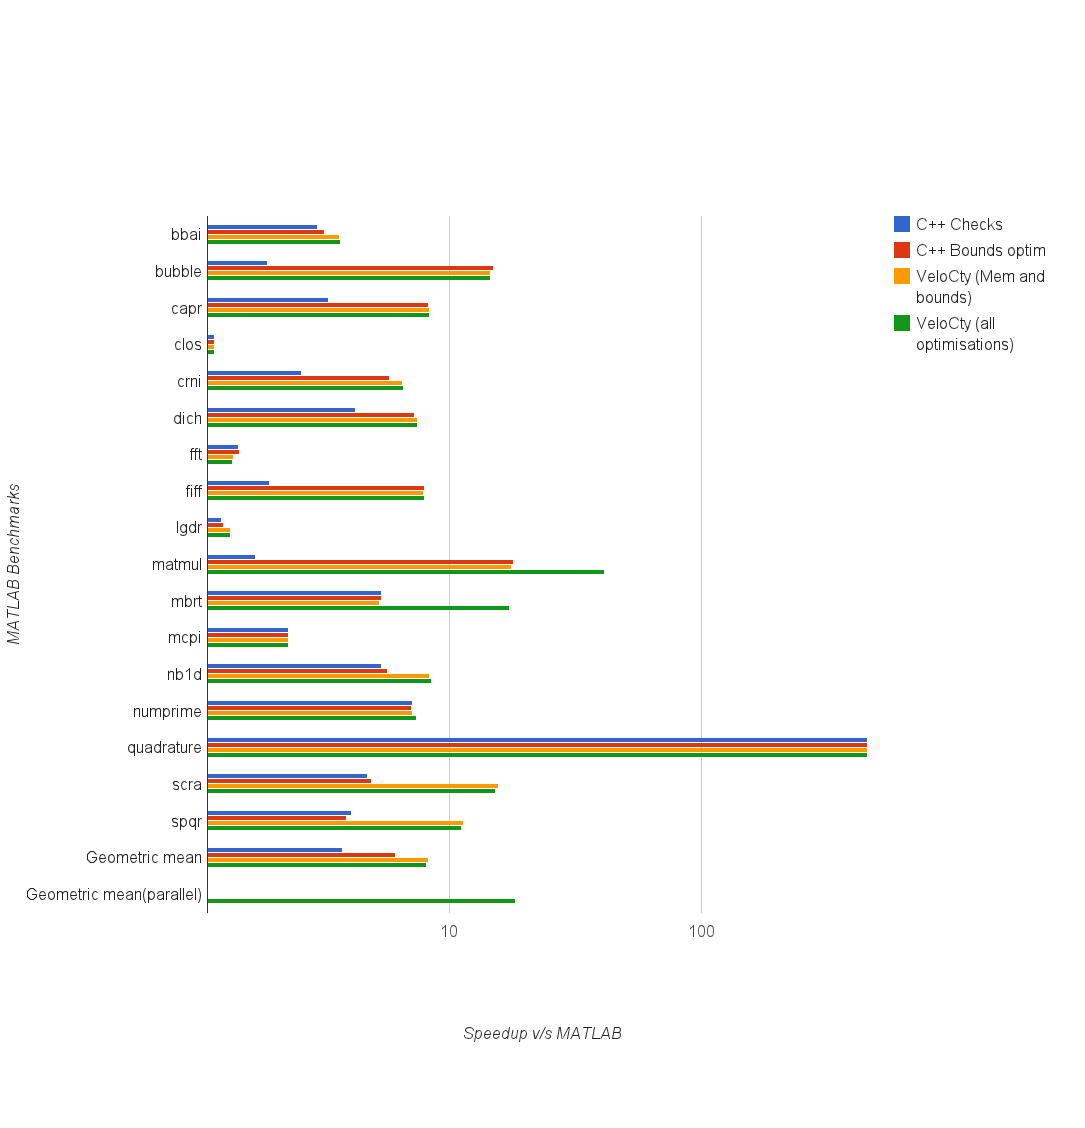
\includegraphics[scale=0.45]{Figures/final_mat.png}
\caption[Summary of \matlab benchmark results]{The figure compares the speedups of different \velocty versions against the Mathworks' interpreter and JIT compiler version for the \matlab benchmarks. Geometric mean(parallel) gives the geometric mean of three benchmarks matmul, mbrt and nb1d when they are executed with all optimisations.}
\label{fig:results_mat}
\end{figure}

As we can observe the we see an increase in the geometric means as we add optimisations. The geometric mean for baseline \velocty is 3.76x, the geomtric mean for the \velocty version with bounds checks optimisations enabled was 6.10x, that for \velocty with bounds checks and memory optimisations was 8.24x and finally the version with all optimisations was 8.5x. In case of the \velocty versions with all the optimisations, if we only consider the three benchmarks that are executed in parallel, we observe a geometric mean of 18.27x.

\section{Python Results}
\subsection{Overall Results}
We ran experiments on 9 Python benchmarks. Similar to the experiments on \matlab benchmarks, we compared the generated VeloCty code without bounds checks to Cython and the CPython interpreter. Figure \ref{fig:results_cwochecks_py} is a bar graph showing the speedup of the generated VeloCty code with checks disabled, the generated VeloCty code with checks enabled and the Cython code compared to the CPython interpreter. The blue bars indicate the speedup of the generated VeloCty code with checks enabled and the red bars indicate the speedup of the Cython code. The geometric mean of the speedups for the generated VeloCty code without checks was 397.17x. The largest speedup of 1281.67x was shown by the \textsf{lud} benchmark. The smallest speedup of 40.98 was shown by the \textsf{fft} benchmark. Note that the Python results are compared against a pure interpreter, C-Python, whereas in case of the \matlab, the results were compared against a interpreter with a JIT compiler. A JIT compiler gives better performance compared to a pure interpreter. Hence we see higher speedups for the \velocty code for Python as compared to the ones we observed for \matlab. 
\begin{figure}[htbp]
\centering
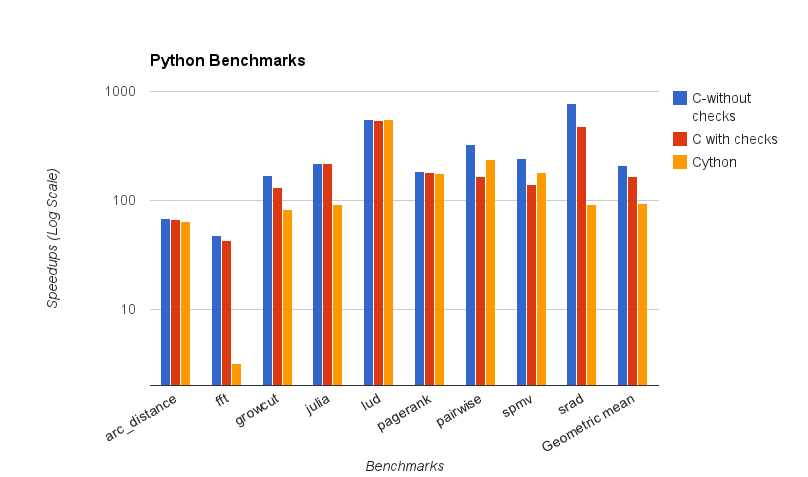
\includegraphics[scale=0.5]{Figures/results_cwochecks_py.png}
\caption{The figure compares the speedups of the \velocty code with all optimisations enabled and and speedups of Cython against the C-Python version for the Python benchmarks.}
\label{fig:results_cwochecks_py}
\end{figure}

The baseline VeloCty code is faster than the Cython code for all the benchmarks. Comparing the speedup of our generated VeloCty code to the Cython code, a mean speedup of 2.21x was found. The largest speedup of 14.93x was shown by the \textsf{fft} benchmark. The benchmarks \textsf{arc\_distance}, \textsf{lud} and \textsf{pagerank} take the same time to execute as our generated C++ code. All three benchmarks have fewer array index operations and more scalar operations compared to the other benchmarks. On the other hand the \textsf{fft} benchmark performs significantly better for the generated VeloCty code than the Cython version. The \textsf{fft} benchmark contains recursive function calls. Cython adds checks to ensure validity of the input arguments of a function as well as validity of the arguments being passed from the function call point. 

\subsection{Impact of Array Bounds Checks on Performance}
Enabling array bounds checks gives a significant slowdown in 4 of the 9 benchmarks. These benchmarks are \textsf{growcut}, \textsf{pairwise}, \textsf{spmv} and \textsf{srad}. Table \ref{tab:cwvscwopy} lists the slowdowns observed for the generated VeloCty versions with checks enabled compared to the generated VeloCty version with checks disabled. The geometric mean of the slowdown is 1.27x. The geometric mean of the slowdown for the affected benchmarks was 1.63. The highest slowdown was shown by the \textsf{pairwise} benchmark. Benchmarks which were not affected by array bounds checks enabled were ones which contained loops with fewer loop iterations or with fewer array index operations in their bodies. 
\begin{table}[htbp]
\centering
\begin{tabular}{|c|c|}
\hline
Benchmarks     & Slowdown    \\ \hhline{|=|=|}
arc\_distance  & 1.02\\ \hline
fft            & 1.09\\ \hline
growcut        & 1.28\\ \hline
julia          & 1.01\\ \hline
lud            & 1.03\\ \hline
pagerank       & 1.01\\ \hline
pairwise       & 1.94\\ \hline
spmv           & 1.73\\ \hline
srad           & 1.64\\ \hline
Geometric mean & 1.26\\ \hline
Geometric mean(Affected Benchmarks)  &  1.63 \\ \hline
\end{tabular}
\caption{Slowdown of the Python benchmarks for VeloCty code with checks enabled compared to VeloCty code without checks}
\label{tab:cwvscwopy}
\end{table}
\subsection{Impact of Bounds Check optimisations on benchmark performance}
We also timed versions of the generated VeloCty code with the bounds check optimisations enabled. We calculated the speedup of \velocty with bounds check optimisations against the baseline \velocty. Table \ref{tab:cwvscopy} lists slowdowns for all the Python benchmarks. The geometric mean of slowdown for the VeloCty code with optimisation is 1.22x. The geometric mean of the speedups of benchmarks which showed a significant speedup is 1.79x. Maximum speedup was of 2.00x and the smallest was of 1.59x. 
\begin{table}[h]
\centering
\begin{tabular}{|c|c|}
\hline
Benchmark      & VeloCty Bounds Check Optimisation \\ \hhline{|=|=|}
arc\_distance  & 1.02                              \\ \hline
fft            & 1.04                              \\ \hline
growcut        & 1.06                              \\ \hline
julia          & 1.01                              \\ \hline
lud            & 1.02                              \\ \hline
pagerank       & 1.02                              \\ \hline
pairwise       & 2.00                              \\ \hline
spmv           & 1.59                              \\ \hline
srad           & 1.60                              \\ \hline
Geometric mean & 1.22                              \\ \hline
\end{tabular}
\caption{Speedup of VeloCty with check optimisation and baseline VeloCty.}
\label{tab:cwvscopy}
\end{table}
\subsection{Impact of parallel execution of VeloCty code}
6 of the 9 benchmarks could be executed in parallel. We calculated the speedups of the VeloCty versions executing in parallel with the baseline VeloCty version. The geometric mean of the speedups was 2.50x. Maximum speedup was observed in the growcut benchmark. The benchmark showed a speedup of 3.96x. The smallest speedup of 2.20x  was observed by the srad benchmark. Table \ref{tab:cpvscwopy} gives the speedups for the 6 benchmarks that could be executed in parallel.
\begin{table}[h]
\centering
\begin{tabular}{|c|c|}
\hline
Benchmark      & VeloCty Parallel \\ \hhline{|=|=|}
arc\_distance  & 1.02             \\ \hline
fft            & 1.04             \\ \hline
growcut        & 3.96             \\ \hline
julia          & 1.01             \\ \hline
lud            & 2.41             \\ \hline
pagerank       & 2.73             \\ \hline
pairwise       & 2.34             \\ \hline
spmv           & 1.83             \\ \hline
srad           & 2.20             \\ \hline
Geometric mean & 1.86             \\ \hline
\end{tabular}
\caption[Speedup of VeloCty parallel for Python]{The table lists the speedups of the VeloCty parallel versions of the Python benchmarks against baseline \velocty code}
\label{tab:cpvscwopy}
\end{table}

\subsection{Summary of Python results}
Figure \ref{fig:results_final} shows a chart with the speedups of the diferent versions of \velocty code for the Python benchmarks compared to the C-Python interpreter. The blue bars represent the speedups of baseline \velocty, the red bars indicate the speedups of the \velocty versions with bounds check optimisations turned on and the yellow bars indicate the speedups of the \velocty versions with bounds check optimisation and parallel code execution. 

\begin{figure}[htbp]
\centering
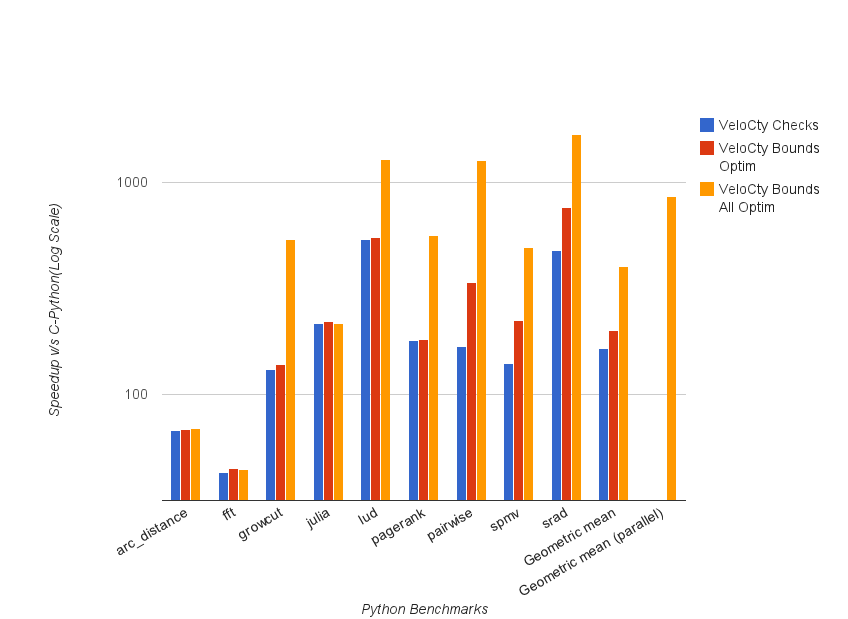
\includegraphics[scale=0.5]{Figures/final_py.png}
\caption[Summary of Python Results]{The bar graph gives the speedups of the \velocty backend for diferent \velocty versions compared to the Mathworks' JIT and VM implemenation. Higher is better. Geometric mean(parallel) gives the speedups of the 6 benchmarks that can be executed in parallel. }
\label{fig:results_final}
\end{figure}

Similar to \matlab we can see the geometric mean of the \velocty versions increasing as we add optimisations. The geometric mean of the baseline \velocty version is 164.48x , the geometric mean of the version with bounds check optimisations enabled is 200.8x and the geometric mean when \velocty code is executed in parallel is 400.98x. The geometric mean of benchmarks which are executed in parallel is 860.09x.

Note that since none of the Python benchmarks contained any array slicing operations or array operations, performance would not differ when the memory optimisation was used and hence we do not specify those numbers in this section. 
\section{Summary}
Through our experiments we showed that compiling `hot' functions of \matlab and Python show significant performance improvement. 
For the \matlab benchmarks, we observed significant  speedups compared to the Mathworks' \matlab interpreter and JIT compiler. We also observed comparable performance with respect to \matlab-coder. We identified bottlenecks in generated code and implemented optimsations, namely the bounds check elimination and the memory optmisation to reduce the impact of the bottlenecks. Due to these optimisations we also observed significant speedups over \matlab-coder for most benchmarks. Moreover we also identified the bottlenecks in the benchmarks which showed poorer performance compared to \matlab-coder and suggested optimisations to eliminate the bottlenecks. The generated code showed significant performance gains for three benchmarks when it was executed in parallel using OpenMP.

On the Python side, we saw very large speedups against the C-Python interpreter. The larger speedup could be attribute to the fact that comparison was against an interpreter without a JIT compiler. We also observed equal or better performance when compared to Cython. The performance of the generated code improved further when the optimisations were added and the code was executed in parallel. 

In conclusion, the VeloCty code with all optimisations enabled generated by \velocty from \matlab is 8.05 times faster than the Mathwork's \matlab. The generated VeloCty code for Python is 400.98 times faster than the C-Python interpreter. We believe that these results are encouraging and have motivated us to further develop the compiler for higher performance gains. 

\chapter{Related Work} \label{chap:Related}
Stuff that's kinda like the stuff I did

\chapter{Conclusions and Future Work} \label{chap:Conclusions}
\section{Conclusions}
The aim of the thesis was to improve performance of array based-languages by compiling computationally intensive code-sections to C++ and then compiling them to a shared library that can be called from the source array-based language. A partial compilation ensures that users can continue writing code in the source language. Another advantage of partial compilation is that portions of code which cannot be compiled ahead of time can be skipped. 

We used the Velociraptor toolkit for implementing the compiler. Velociraptor provides language agnostic tools and analyses to aid generation of high-performance code. The Velociraptor intermediate representation, VRIR, is a high-level AST based representation which has semantics that are close to those of array-based languages. This makes writing a front-end compiler to VRIR easy. Moreover, VRIR has flexible semantics to accommodate the semantic differences of different array-based languages. This allows us to write a single backend to compile from VRIR to C++, which can be used for multiple array-based languages. VRIR also contains constructs such as parallel for, map and reduce statements which can be used to generate parallel code. Additionally, Velociraptor provides analyses and transformations which aid in code generation. 

Contributions of this thesis can be divided into four parts. The first is the implementation of a frontend for the \matlab language. The frontend was implemented using the open source \mclab toolkit. We faced challenges while compiling from a \matlab-specific intermediate representation to a language agnostic one. Determining the types of the expression nodes in VRIR and converting a colon expression to a range expression include some of them. The second is the generation of the glue code that is required to interface the generated code with \matlab. This involved the generation of code that converts \matlab-specific arrays to \velocty arrays, calling the generated function and finally converting the \velocty arrays back to the \matlab-specific array. The implementation of a compiler backend from VRIR to C++ is the third contribution of this thesis. The code generator was flexible enough to generate C++ code for the different semantics supported by VRIR. For example, the code generator can generate code for both row major and column major arrays. Additionally, we implemented runtime libraries for both \matlab and Python. These libraries implement different builtin functions supported by both languages, array bounds checks and array slicing operations among other functions. The final contribution of the thesis was to optimise the generated code. We implemented optimization to eliminate bounds checks inside loop bodies and eliminated redundant unnecessary memory allocations during array operations. Also, we supported naive parallelism using OpenMP.  

We observed significant gains in performance when comparing the generated code against the standard implementations for \matlab and Python, the Mathworks' \matlab interpreter and JIT compiler and the CPython interpreter respectively. We also observed gains over other tools for performance improvement for these languages such as the \matlab-coder for \matlab and Cython for NumPy.  

In conclusion, we would like to state that \velocty does achieve significant performance gains for both \matlab and NumPy. We believe that partial compilation improves usability by allowing users to continue using their preferred scientific language. Finally, our compiler backend is language agnostic and can help compiler writers improve performance of other languages such as R and Julia. \velocty is open source and freely available and hence can be reused and modified by researchers for their own work. 

\section{Future Work}
Although \velocty does achieve significant performance gains, there still is scope for improvement. We see five areas where improvement in performance may be achieved.
\subsection{Automatic detection of computationally intensive code sections}
In the current implementation of \velocty, we depend on the user to identify and annotate code sections, which can then be compiled to C++. In the future, the implementation could be improved to automatically identify computationally intensive code sections and compile them to C++. 
\subsection{GPU code generation}
Heterogeneous architectures are gaining popularity in recent times. Many low-level languages and libraries have been developed for writing code for these architectures. These languages make good targets for high-performance compilers. An enhancement of \velocty could be the generation of GPU code from the parallel for loops. 
\subsection{Auto-parallelization}
\velocty currently supports naive parallelism. The user has to annotate the parallel for loops with a list of variables that are shared inside the loop. A possible improvement to \velocty would be the implementation of algorithms that automatically identify loops which can be executed in parallel and identify the list of variables that are shared and ones that are private. Another improvement would be identification of statements that can be vectorised and replacing the statements by vector instructions. 
\subsection{Optimisations}
Many optimisations can be performed on the generated code to improve its performance. The \matlab frontend can be optimised to eliminate copy statements and copies of arrays  during function calls when the arrays are being written to. The bounds check optimisation can be improved to support a larger range of loops and indices. Additionally, operations on arrays can be made lazy and can only be performed when the array elements are accessed. This optimisation may lead to performance gains, since if a chain of array operations are performed, memory can be reused across operations. 
\subsection{Faster Builtins}
The builtin functions in the runtime libraries have naive implementations. Many techniques such as parallelism and vector instructions can be used to improve the performance of these functions. 
\subsection{Readability}
The aim of the thesis was to ensure correct compilation of optimised code for \matlab and NumPy. In the future, we would like to add information to the generated code which would improve readability and simplify debugging of code. One approach could be to add the line numbers of the original code from which a certain code section has been generated. 


% -- Bibliography -------------------------------------------------------------

%\addtocontents{toc}{\protect\addvspace{10pt}}

%\bibliographystyle{plain}

\bibliographystyle{web-alpha} %- originally in jesse thesis
%\bibliography{strings, thesis}
\bibliography{refs}


\appendix % -- Appendices -----------------------------------------------------

% -- Glossary & Index ---------------------------------------------------------

%\addtocontents{toc}{\protect\addvspace{10pt}}
%\include{text/appendices/Glossary}
%\include{text/appendices/Index}

\end{document}

